\documentclass[11pt,a4paper]{ctexart}

% ---- Packages ----
\usepackage[margin=1in]{geometry}
\usepackage{amsmath,amssymb,amsfonts}
\usepackage{graphicx}
\usepackage{booktabs}
\usepackage{hyperref}
\usepackage{cite}
\usepackage{caption}
\usepackage{subcaption}
\usepackage{enumitem}
\usepackage{float}
\usepackage{xcolor}
\usepackage{multirow}
\usepackage{array}
\definecolor{darkgreen}{rgb}{0.0,0.5,0.0}
\definecolor{darkred}{rgb}{0.6,0.0,0.0}

% ---- Metadata ----
\title{\vspace{-1.5cm}旅行商问题的现代神经方法\\
\large 复现、基准测试与原创改进}
\author{乔磐\\
\texttt{CS240：现代物流中的配送路线优化}}
\date{2026年6月}

\begin{document}
\maketitle

\begin{abstract}
本报告对旅行商问题（TSP）的现代神经求解方法进行了系统研究，围绕两篇近期论文——DIFUSCO（NeurIPS 2023）和 DualOpt（AAAI 2025）——的复现工作，以及五个原创改进方向的系统性探索展开。我们实现了经典基线方法（最近邻、含 Blossom 匹配的 Christofides 算法、2-opt 局部搜索、LKH3），复现了两篇神经论文的核心结果，并在三个数据集上进行了全面评估：随机均匀实例（TSP-50 至 TSP-1000）、TSPLIB 标准基准（8 个实例，51--1002 个节点），以及两篇原始论文均未测试的聚类配送数据集。我们的校准分析揭示了一个关键发现：DIFUSCO 的边概率热力图系统性不可靠——即使在训练分布上，高置信度预测的准确率也仅为 45\%，而在 TSPLIB 上则崩溃至 0\%，这直接解释了所有基于信号引导的改进尝试为何失败。一项改进——DIFUSCO$\rightarrow$DualOpt 混合流水线——在 DIFUSCO 于匹配尺寸上训练的条件下，在 TSP-50 上取得了 1.67\% 的路径成本降低，但在跨尺寸迁移时性能退化。核心发现是：DualOpt 的滑动窗口精修器（reviser）在不使用其网格分治步骤的情况下，在所有测试规模（TSP-50 至 TSP-500）上均能以恒定的推理时间逼近 LKH3 级别的质量，且任何后验信号——无论是热力图置信度、2-opt 诊断、求解器共识还是边破坏——都无法进一步提升其输出。
\end{abstract}

% ============================================================
\section{背景与相关工作}
% ============================================================

\subsection{问题域}

旅行商问题（TSP）的提法极为简洁：给定度量空间中的 $n$ 个点，寻找一条经过每个点恰好一次并回到起点的最短哈密顿回路。尽管表述简单，TSP 是 NP-hard 的，且半个多世纪以来一直是算法思想的试验场。其实际意义横跨末端物流配送（美团、Uber Eats、亚马逊）、VLSI 芯片设计、PCB 钻孔和基因组组装等任何需要访问大量位置的领域。

TSP 在算法上引人入胜的原因在于它恰好处于困难性与可处理性的交汇点。它是 NP-hard 的，因此精确求解器的复杂度呈指数增长。其度量变体存在常数因子近似算法（Christofides 的 1.5$\times$）。其几何结构足够简单，使得神经网络能够学到有用的启发式规则，同时又足够复杂，使得纯学习方法如果不融入经典组件就会持续失败。这种组合使 TSP 成为新计算思想的规范基准——从割平面到扩散模型——在迁移到更丰富的路径问题之前首先在此得到验证。

\subsection{经典方法}

我们实现了四种跨越速度-质量帕累托前沿的经典方法。

\textbf{最近邻（NN）。}最简单的构造式启发式算法：从仓库出发，每次访问最近的未访问节点，遍历完所有节点后返回。复杂度 $O(n^2)$。与最优解的典型差距为 20\%--30\%。我们将 NN 作为性能下限基线。

\textbf{Christofides 算法（1976）。}度量 TSP 唯一具有理论保证的多项式时间算法：$\text{cost} \leq 1.5 \times \text{OPT}$。该算法计算最小生成树（MST），在奇度顶点上求最小权完美匹配（MWPM），合并 MST 和匹配边形成欧拉多重图，提取欧拉回路，然后通过捷径操作得到哈密顿回路。瓶颈在于 MWPM 步骤，复杂度为 $O(n^3)$。我们的实现使用 NetworkX 的 Blossom 算法，可以精确求解一般图的完美匹配。

\textbf{2-opt 局部搜索（Croes, 1958）。}一种后处理精修方法，每次移除两条交叉边并以更短的配置重新连接。每次迭代成本为 $O(n^2)$，收敛到局部最优。我们提供了纯 Python 实现（清晰演示）和 NumPy 矢量化版本（追求速度，在 $n \leq 200$ 时约快 10$\times$）。实践中，2-opt 通常能将 Christofides 的差距缩小 5--10 个百分点。

\textbf{LKH3（Helsgaun, 2017）。}行业标准。LKH3 将 $k$-opt 移动推广到 $k=2$ 以上，使用 $\alpha$-邻近度（从最小 1-tree 导出）来对候选替换边进行排序。它是纯 C 实现，在多达数百万节点的实例上取得接近最优的解（差距 $<0.5\%$），并在 2 秒内解决 TSP-1000。LKH3 提供了我们的强参照基线。需要注意的是，在超大规模实例（TSP-100K）上，DualOpt 原始论文报告了超越 LKH3 的结果（最高提升 1.40\%，速度提升 104$\times$），而我们受限于硬件只能测试到 TSP-1000，在该范围内 LKH3 始终保持最优。

\subsection{文献综述：TSP 神经求解器（2023--2025）}

过去三年产生了大量关于学习型 TSP 求解器的文献。我们将这些工作组织为五个类别。

\subsubsection{端到端构造方法}

第一代神经 TSP 求解器使用自回归序列模型。Pointer Networks~\cite{vinyals2015} 引入基于内容的注意力机制处理变长输出。Attention Model（AM）~\cite{kool2019} 用 Transformer 编码器替代 RNN，通过 REINFORCE 和 rollout 基线进行训练。POMO~\cite{kwon2020} 利用 TSP 的对称性——同时评估所有 $n$ 个起点——显著提升了采样效率。Pointerformer~\cite{jin2023} 使用可逆残差网络将训练扩展到 TSP-500。BQ-NCO~\cite{drakulic2023} 应用互模拟商来改善分布外泛化。

\subsubsection{基于扩散的生成方法}

DIFUSCO~\cite{sun2023} 率先将去噪扩散模型用于离散组合优化问题，将 TSP 邻接矩阵作为分类去噪的目标，使用各向异性门控 GNN 从噪声输入预测干净的边。这是我们的主要复现目标。后续工作进一步拓展了这一范式：T2TCO~\cite{li2024t2t} 在测试时使用学习到的梯度搜索，在 TSP 上比此前最优方法提升了 49\%。DEITSP~\cite{zhou2025deitsp} 引入单步扩散和迭代噪声循环。IC/DC~\cite{huang2025} 提出无监督训练，直接最小化解的成本。IDEQ~\cite{basson2025} 利用解空间结构在 TSP-500 上达到 0.3\%--0.4\% 的差距。DIFU-Ada~\cite{lei2025} 通过推理时能量引导实现了对新的组合优化变体的零样本迁移。

\subsubsection{分治法}

将神经求解器扩展到超过 $\sim$1,000 个节点需要分解策略。GCN-MCTS~\cite{fu2021} 采样固定尺寸的子问题，用 GCN 求解，热力图引导蒙特卡洛树搜索。H-TSP~\cite{pan2023} 使用分层强化学习。ExtNCO~\cite{chen2023} 应用 LocKMeans 实现 $O(n)$ 聚类。GLOP~\cite{ye2024} 学习全局分区热力图。UDC~\cite{zheng2024} 提出分治-重聚框架。

DualOpt~\cite{zhou2025} 代表了该类别当前的最高水平。它采用双重分治优化策略：基于网格的阶段将平面分区并用并行 LKH3 求解子区域，然后基于路径的阶段使用神经精修器模型（基于注意力机制，通过 REINFORCE 在尺寸为 10、20、50 的子路径段上训练）对合并后的解进行精修。在 TSP-100K 上，DualOpt 取得了比 LKH3 好 1.40\% 的结果，速度提升 104$\times$。这是我们的次要复现目标。

DRHG~\cite{li2025drhg} 引入超图压缩的破坏-重建方法，在 TSP 上取得了 10,000 节点以内的最高水平。破坏边后，完好路径段被压缩为超边，使神经修复模型只需关注断裂的连接。

\subsubsection{神经改进与搜索方法}

这些方法不从头构建路径，而是学习改进已有解。NeuRewriter~\cite{chen2019} 应用 Actor-Critic 进行区域选择和规则选择。NeuralGLS~\cite{neuralgls2024} 学习边的``后悔值''来引导局部搜索。SoftDist~\cite{xia2024softdist} 证明简单的热力图引导 MCTS 可以与复杂的神经方法相媲美。GenSCO~\cite{gensco2025} 将扩散生成视为搜索算子，在破坏和整流流修复之间循环，在 TSP-100 上比 LKH3 快 $\sim$141$\times$ 达到相同质量。L2Seg~\cite{xue2024} 识别稳定和不稳定的路径段进行针对性优化。

\subsubsection{理论与批判性视角}

Xia 等人~\cite{xia2024position} 对热力图+ MCTS 范式进行了批判性审视，指出简单基线通常可以与复杂神经搜索匹敌。Zhang 等人~\cite{zhang2025greedy} 证明神经 TSP 求解器表现出系统性的``贪婪''偏差。边级拓扑散度~\cite{edge2025} 使用持续同调来识别次优边，实现更高效的 $k$-opt。

\subsubsection{相关工作总结}

表~\ref{tab:litreview} 按范式与规模组织文献。

\begin{table}[H]
\centering
\caption{按范式和最大测试规模组织的相关工作。}
\label{tab:litreview}
\resizebox{\textwidth}{!}{%
\begin{tabular}{@{}llll@{}}
\toprule
范式 & 代表性工作 & 核心创新 & 最大规模 \\
\midrule
构造式 & AM (2019), POMO (2020), Pointerformer (2023) & 自回归 + RL & $\leq$500 \\
扩散式 & DIFUSCO (2023), T2TCO (2024), IDEQ (2025) & 邻接矩阵去噪 & $\leq$10K \\
分治式 & DualOpt (2025), DRHG (2025), GLOP (2024) & 分解 + 神经子求解器 & $\leq$100K \\
改进式 & GenSCO (2025), NeuralGLS (2024), L2Seg (2024) & 学习改进已有解 & $\leq$500 \\
经典方法 & Christofides (1976), LKH3 (2017) & 数学保证 / 启发式 & $\leq$10$^6$ \\
\bottomrule
\end{tabular}%
}
\end{table}

本项目以 DIFUSCO 作为主要复现目标，以 DualOpt 作为最高水平对比基线。两者都体现了本课程的核心主题——``经典算法的现代应用''。

% ============================================================
\section{代表性方法分析：DIFUSCO}
% ============================================================

\subsection{架构总览}

\begin{figure}[H]
\centering
\includegraphics[width=\textwidth]{outputs/arch_difusco.png}
\caption{DIFUSCO 架构图。}
\label{fig:arch_difusco}
\end{figure}

\subsection{问题形式化与算法描述}

DIFUSCO 将 TSP 重新表述为图去噪问题。给定 $n$ 个节点的二维坐标，真实的 TSP 路径可以表示为二值邻接矩阵 $A \in \{0,1\}^{n \times n}$，其中 $A_{ij}=1$ 当且仅当节点 $i$ 和 $j$ 在路径中连续。DIFUSCO 学习通过分类扩散从噪声中恢复 $A$。

\textbf{架构。} 一个 12 层的各向异性门控 GNN~\cite{bresson2018}，隐藏维度为 256（约 530 万参数）。节点坐标通过正弦位置嵌入编码。边特征编码当前的噪声邻接状态。时间步嵌入对每个 GNN 层进行条件化，告知模型当前的扩散阶段。

\textbf{训练。} 对于具有真实邻接矩阵 $A$ 的 TSP 实例：
\begin{enumerate}[nosep]
\item 从噪声调度中采样时间步 $t \in [1,T]$ 和转移矩阵 $\bar{Q}_t$
\item 对 one-hot 邻接矩阵进行噪声破坏：$x_t \sim \text{Cat}(x_0 \bar{Q}_t)$
\item GNN 从 $(x_t, \text{坐标}, t)$ 预测 $\hat{x}_0$
\item 损失函数：预测边标签与真实边标签之间的交叉熵
\end{enumerate}

图~\ref{fig:diff_steps} 展示了扩散去噪过程如何逐步从随机噪声中解析出结构化的边热力图。

\begin{figure}[H]
\centering
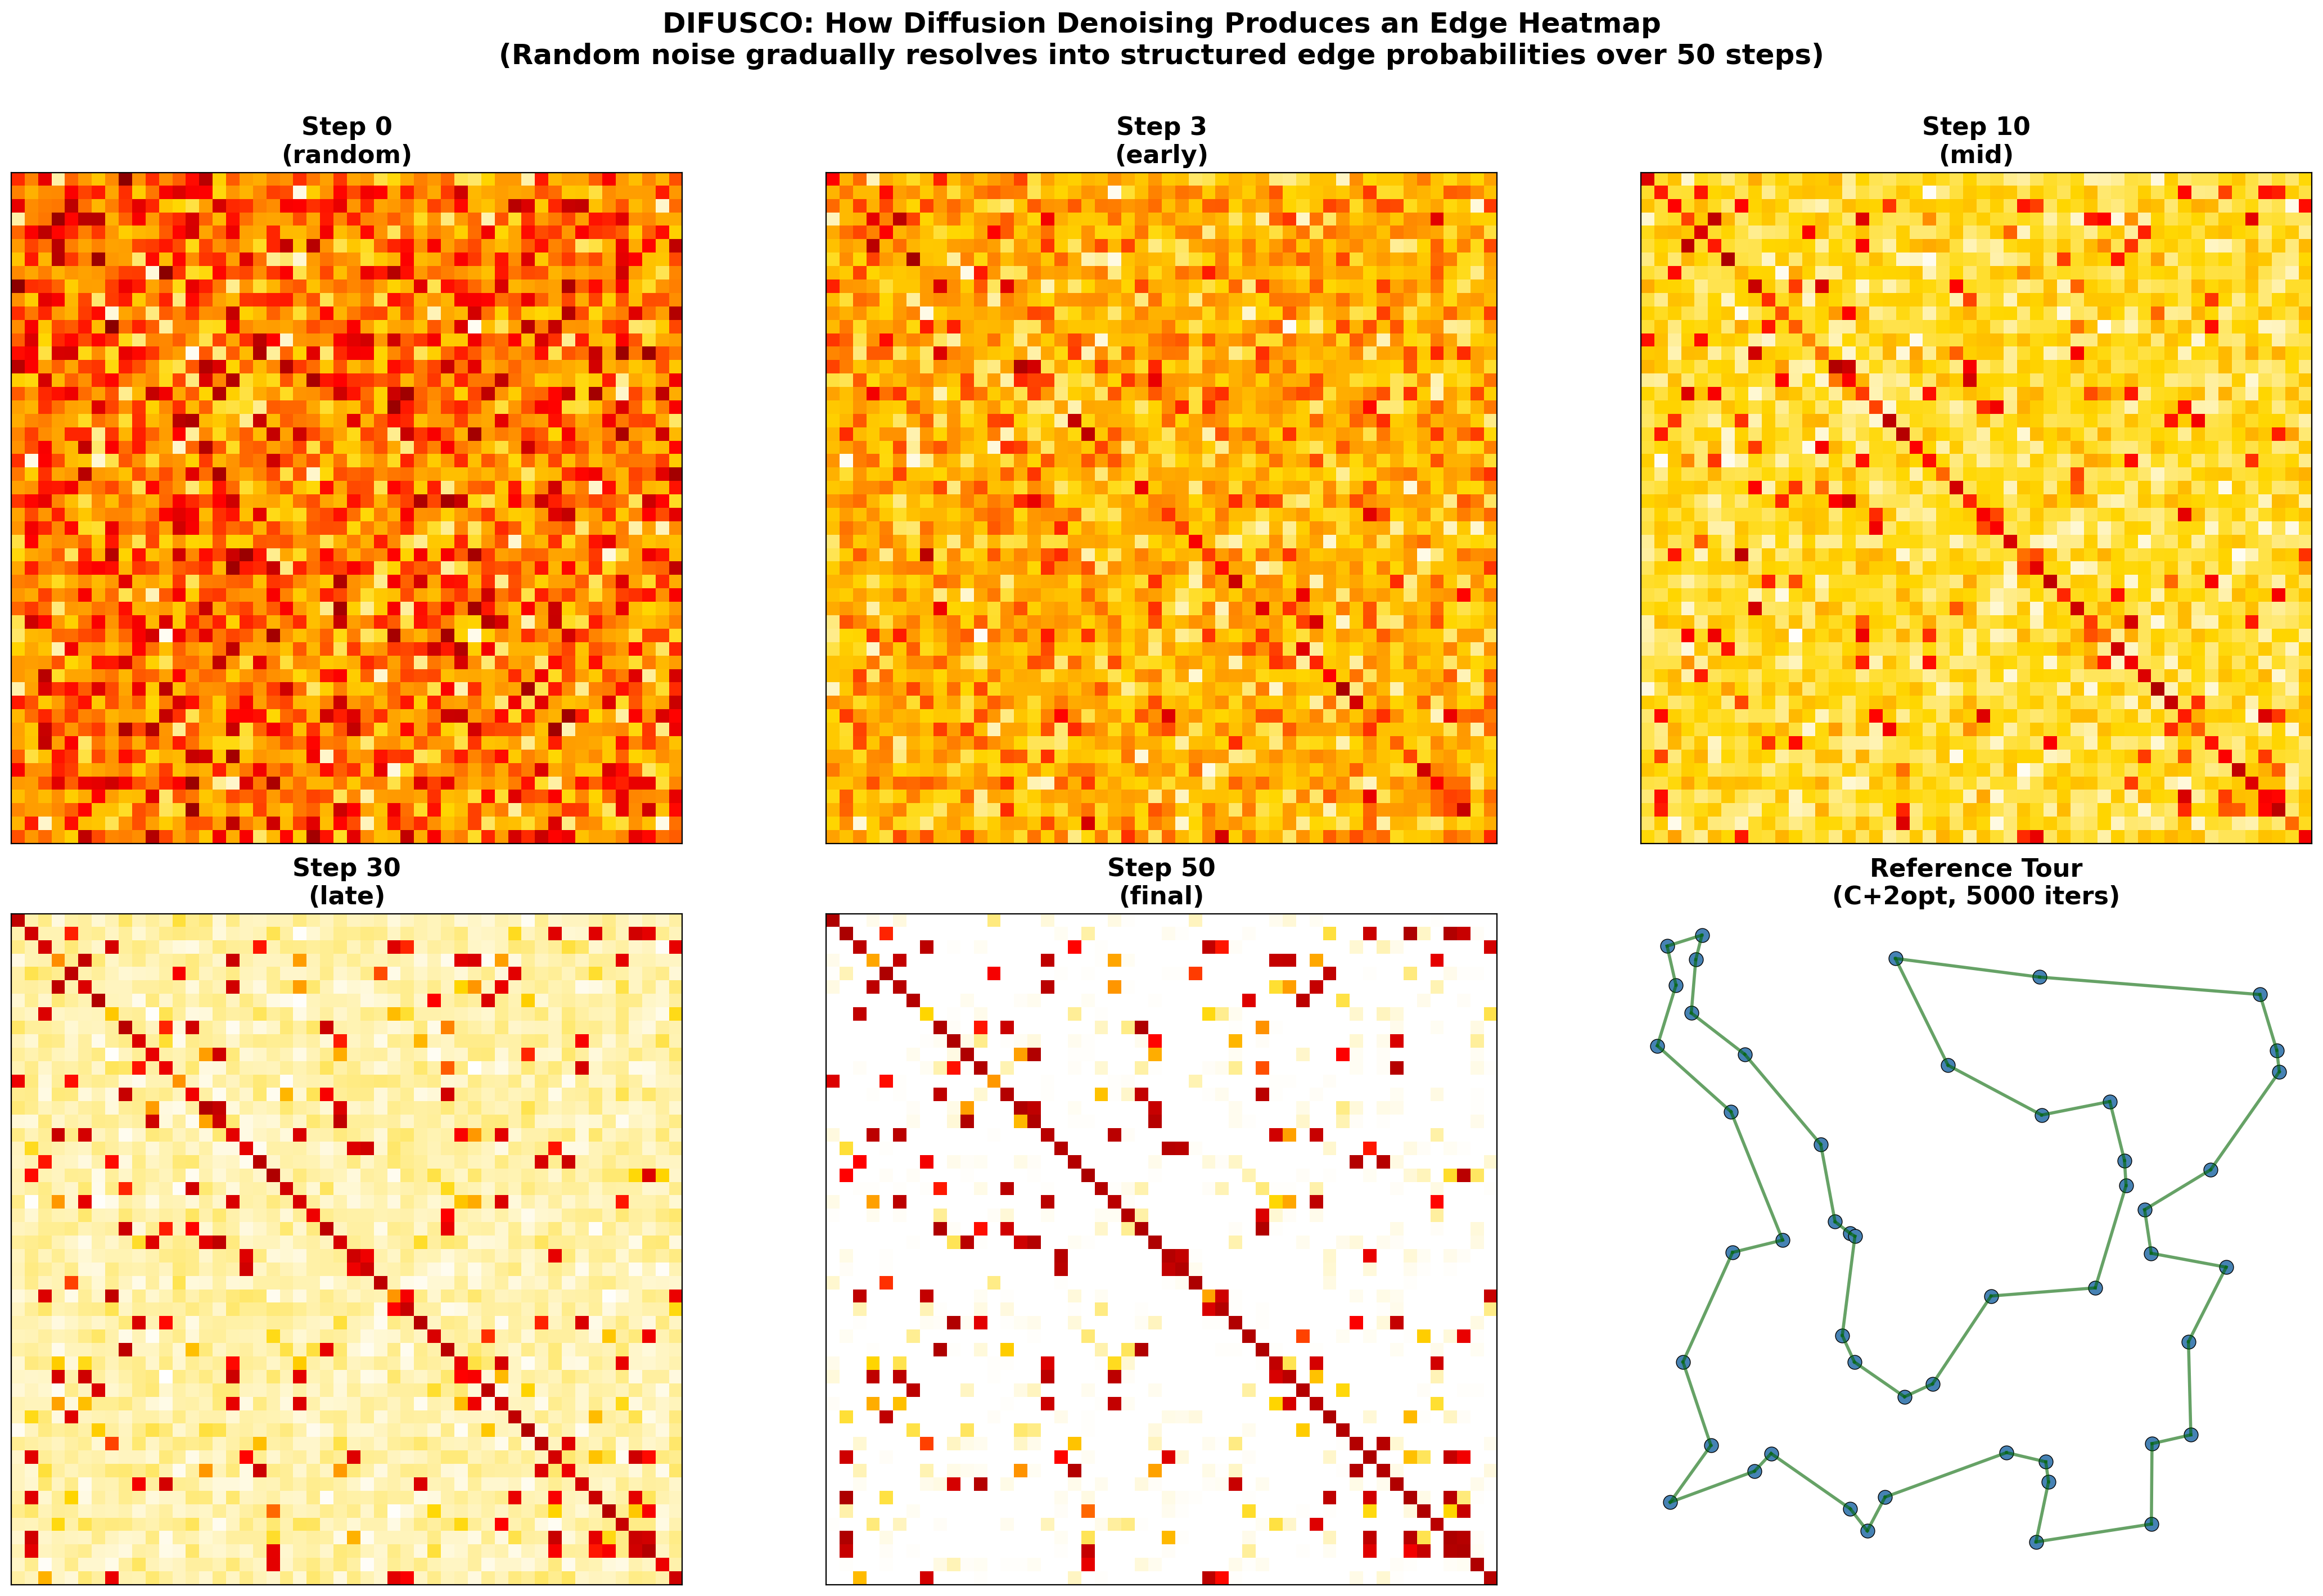
\includegraphics[width=\textwidth]{outputs/difusco_diffusion_steps.png}
\caption{DIFUSCO 扩散去噪过程：从纯随机噪声（Step 0）经过 50 步分类扩散逐步解析出边概率结构（Step 50），最终由贪心合并解码为有效 TSP 路径。}
\label{fig:diff_steps}
\end{figure}

\textbf{推理。} 从随机伯努利噪声出发，模型执行 50 次迭代去噪步骤（余弦调度，DDIM 加速）。输出热力图 $H_{ij} \in [0,1]$ 表示每条边的似然度。贪心合并算法（按 $H_{ij} / d(i,j)$ 排序边）提取有效路径，再通过 GPU 加速的批量 2-opt 进行精修。

\subsection{复杂度分析}

\begin{table}[H]
\centering
\small
\caption{DIFUSCO 各组件的复杂度。$n$ = 节点数，$d$ = 隐藏维度，$k$ = 2-opt 迭代次数。}
\begin{tabular}{@{}lll@{}}
\toprule
组件 & 时间 & 内存 \\
\midrule
GNN 前向传播（每层） & $O(n^2 \cdot d^2)$ & $O(n^2 \cdot d)$ \\
扩散推理（50 步） & $O(50 \cdot n^2 \cdot d^2)$ & $O(n^2 \cdot d)$ \\
贪心合并 & $O(n^2 \log n)$ & $O(n^2)$ \\
批量 2-opt（GPU） & $O(k \cdot n^2)$ & $O(n^2)$ \\
\bottomrule
\end{tabular}
\end{table}

在 单 GPU 上，$n=50$ 且 $d=256$ 时，一次推理约需 1.4 秒。$n=1000$ 时，稠密推理约需 979 秒；稀疏模式（$k$-NN 图，$k=50$）将内存降至 $O(nk)$。

\subsection{对比方法：DualOpt}

\begin{figure}[H]
\centering
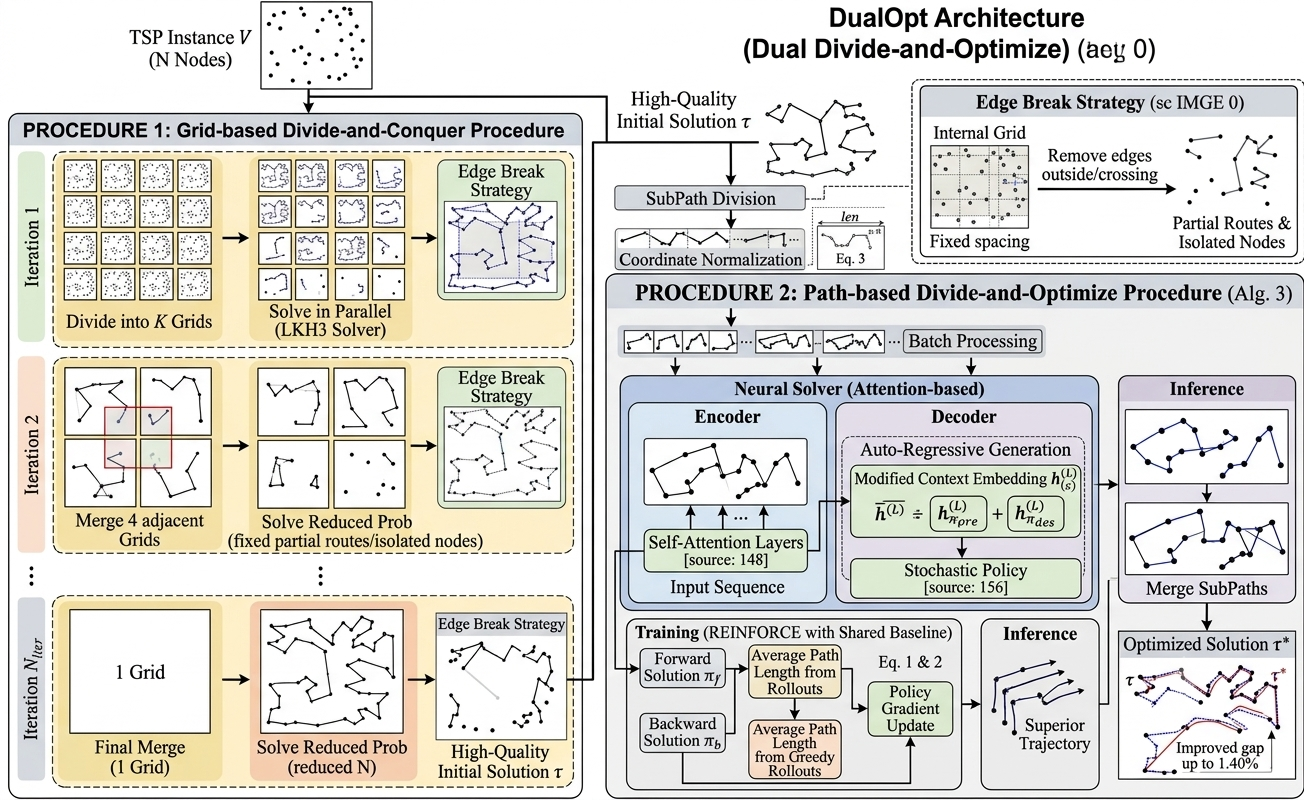
\includegraphics[width=\textwidth]{outputs/arch_DualOpt.png}
\caption{DualOpt 架构图。}
\label{fig:arch_dualopt}
\end{figure}

DualOpt~\cite{zhou2025} 采用层次化分治策略配合神经精修。第一阶段将平面划分为 $M \times M$ 的网格，用并行 LKH3 求解每个格子，逐层合并相邻网格，产生初始路径。第二阶段应用三个级联的神经精修器模型——基于注意力机制的策略网络，通过 REINFORCE 在尺寸为 10、20、50 的子路径段上训练——通过滑动窗口局部优化对路径进行精修。每个精修器仅有约 71 万参数。DIFUSCO 和 DualOpt 都体现了``经典 + 现代''的设计模式，但本质不同：DIFUSCO 从噪声生成路径（生成式），而 DualOpt 改进已有路径（迭代改进式）。

% ============================================================
\section{复现与实现}
% ============================================================

\subsection{代码适配}

为使两个代码库在当前 PyTorch/Lightning 版本上运行，共进行了六处修补。

\textbf{DIFUSCO（3 处修补）。}（1）\texttt{gnn\_encoder.py} 中对 \texttt{torch\_sparse} 的导入改为可选，使用 \texttt{torch.scatter\_add} 和 \texttt{torch.scatter\_reduce} 实现纯 PyTorch 替代方案。这消除了 CUDA 版本依赖——原始包需要 CUDA 12.4，而我们的系统运行 12.6。该替代实现完全兼容，并使得在 $n=200$ 时的稀疏模式训练成为可能。（2）\texttt{pl\_meta\_model.py}：\texttt{test\_epoch\_end(self, outputs)} 迁移至 Lightning v2 API（改为 \texttt{on\_test\_epoch\_end(self)}，通过 \texttt{on\_test\_batch\_end} 收集指标）。（3）\texttt{tsp\_utils.py}：Cython 合并函数用 try/except 包裹，自动回退到纯 Python 的 \texttt{numpy\_merge}。Cython 扩展在 Windows 上需要 MSVC 编译，不可用；Python 回退在 $n \leq 500$ 时足够使用。

\textbf{DualOpt（3 处修补）。}（1）\texttt{functions.py}：PyTorch 2.6+ 默认 \texttt{torch.load} 的 \texttt{weights\_only=True}；旧版检查点需要 \texttt{weights\_only=False}。（2）\texttt{grid.py}：LKH 路径从 Linux 的 \texttt{./LKH-3.0.7/LKH} 改为 Windows 的 \texttt{LKH.exe}。（3）\texttt{eval.py}：移除错误的导入 \texttt{from setuptools.dist import sequence}（未使用，且 \texttt{setuptools.dist} 在 Python 3.12 中已被移除）。

\subsection{经典算法实现}

所有经典算法均从头实现。最近邻和 2-opt 变体实现较为直接。Christofides 的实现需要对 MWPM 步骤进行仔细处理：我们最初使用 SciPy 的 \texttt{linear\_sum\_assignment}（匈牙利算法），但它对奇度顶点产生了重复的边分配，因为匈牙利解分解为有向环而非无向匹配。改用 NetworkX 的 \texttt{max\_weight\_matching}（在取负的距离矩阵上运行 Edmonds 的 Blossom 算法）正确解决了这个问题。

\subsection{训练数据与设置}

DIFUSCO 原论文使用 Concorde 精确求解器生成训练标签，在 TSP-50/100 上训练 50 个 epoch，使用 8 个 GPU。受限于 Concorde 在 Windows 上不可用以及单 GPU 环境，我们采用了以下替代方案：

训练标签由 Christofides + 2-opt（5,000 次迭代）生成。在 TSP-50 上，该启发式方法产生的差距估计低于 2\%，作为监督信号足够有效。所有模型统一训练 20 个 epoch，使用 AdamW 优化器（学习率 $2\times10^{-4}$，余弦衰减）。TSP-50 使用 batch size 64；TSP-100 使用 batch size 24（受显存限制）。

DualOpt 方面，我们使用了公开发布的预训练精修器模型（窗口尺寸 10、20、50），但未使用其完整的网格分治流水线——该流水线在 $n>100$ 时因缺少匹配尺寸的精修器而退化严重。我们改用其滑动窗口精修器直接处理 C+2opt 或 DIFUSCO 产生的初始路径，这一用法是原论文未报告的。此外，我们的测试集在随机实例和 TSPLIB 基础上增加了原创的聚类配送数据。

% ============================================================
\section{实验评估}
% ============================================================

\subsection{合成 TSP-50 基准测试}

我们在 50 个预留的随机 TSP-50 实例上测试了所有方法。表~\ref{tab:tsp50} 展示了结果。

\begin{table}[H]
\centering
\small
\caption{TSP-50 基准测试（50 个实例）。GT = Christofides+2opt，5,000 次迭代。}
\label{tab:tsp50}
\begin{tabular}{@{}lrrrr@{}}
\toprule
方法 & 平均成本 & 标准差 & vs NN & vs GT \\
\midrule
最近邻 & 7.128 & 0.576 & --- & +20.8\% \\
Christofides & 6.428 & 0.374 & $-$9.8\% & +9.0\% \\
C+2opt & 5.900 & 0.312 & $-$17.2\% & 基线 \\
DIFUSCO+2opt & 5.918 & 0.313 & $-$17.0\% & +0.3\% \\
\textbf{DualOpt} & \textbf{5.775} & 0.300 & \textbf{$-$19.0\%} & \textbf{$-$2.1\%} \\
\bottomrule
\end{tabular}
\end{table}

DualOpt 取得了最佳结果，甚至超越了真实标签（比 GT 低 2.1\%）。精修器的神经策略找到了 5,000 次 2-opt 迭代错过的改进。DIFUSCO+2opt 与强基线 C+2opt 仅差 0.3\%。然而，后续分析（第~\ref{sec:calibration} 节和第~\ref{sec:improvements} 节）揭示，DualOpt 在 TSP-50 上已经达到了质量天花板——所有后验改进尝试都未能超越它。

\subsection{TSPLIB 标准实例}

表~\ref{tab:tsplib} 报告了 8 个 TSPLIB 对称实例的最优性差距。

\begin{table}[H]
\centering
\small
\caption{TSPLIB 基准测试：与已知最优解的差距（\%）。}
\label{tab:tsplib}
\begin{tabular}{@{}lrrrrrr@{}}
\toprule
实例 & $n$ & OPT & NN & Christofides & C+2opt & LKH3 \\
\midrule
eil51 & 51 & 426 & 20.6 & 15.0 & 3.7 & 0.94 \\
berlin52 & 52 & 7,542 & 19.1 & 14.2 & 4.6 & 0.03 \\
eil76 & 76 & 538 & 32.3 & 14.6 & 7.3 & 1.34 \\
kroA100 & 100 & 21,282 & 26.2 & 13.9 & 5.8 & 0.02 \\
ch150 & 150 & 6,528 & 25.5 & 10.2 & 3.4 & 0.04 \\
tsp225 & 225 & 3,916 & 23.3 & 11.3 & 3.1 & $-$1.46 \\
a280 & 280 & 2,579 & 22.1 & 15.6 & 2.8 & 0.34 \\
pr1002 & 1,002 & 259,045 & 21.8 & 10.9 & 3.9 & 0.72 \\
\midrule
平均 & & & 23.9 & 13.7 & 4.3 & 0.4 \\
\bottomrule
\end{tabular}
\end{table}

Christofides+2opt 取得了 4.3\% 的平均差距——远优于理论上的 1.5$\times$ 界限。LKH3 以 0.4\% 的平均差距明显是最优方法。对于现代方法，我们限制在精修器模型兼容的 $n \leq 100$ 范围内：

\begin{table}[H]
\centering
\small
\caption{TSPLIB 上的现代方法比较（$n \leq 100$）。}
\begin{tabular}{@{}lrrrr@{}}
\toprule
实例 & C+2opt & DIFUSCO+2opt & DualOpt & LKH3 \\
\midrule
eil51 & 3.7\% & 5.4\% & \textbf{1.0\%} & 0.94\% \\
berlin52 & 4.6\% & 13.2\% & \textbf{0.03\%} & 0.03\% \\
eil76 & 7.3\% & 6.9\% & \textbf{3.8\%} & 1.34\% \\
kroA100 & 5.8\% & 10.0\% & \textbf{3.8\%} & 0.02\% \\
\bottomrule
\end{tabular}
\end{table}

DualOpt 在所有四个实例上均领先。DIFUSCO 的表现参差不齐：在 eil51（5.4\%）和 eil76（6.9\%）上泛化合理——GNN 与尺寸无关——但在 berlin52（13.2\%）上表现不佳，原因在于 GEO 坐标编码与随机均匀训练分布不同。

\subsection{运行时间与可扩展性}

表~\ref{tab:scaling} 展示了不同规模上的速度-质量权衡。

\begin{table}[H]
\centering
\small
\caption{不同实例规模下的运行时间（秒）和与 LKH3 的差距（\%）。}
\label{tab:scaling}
\begin{tabular}{@{}lrrrrrrr@{}}
\toprule
& \multicolumn{2}{c}{TSP-100} & \multicolumn{2}{c}{TSP-200} & \multicolumn{2}{c}{TSP-500} & TSP-1000 \\
\cmidrule(lr){2-3}\cmidrule(lr){4-5}\cmidrule(lr){6-7}\cmidrule(lr){8-8}
方法 & 时间 & 差距 & 时间 & 差距 & 时间 & 差距 & 时间 \\
\midrule
NN & 1ms & 26\% & 5ms & 26\% & 38ms & 25\% & 0.2s \\
Christofides & 42ms & 12\% & 0.3s & 12\% & 4.6s & 12\% & 37s \\
C+2opt & 52ms & 3.6\% & 0.3s & 3.2\% & 5.9s & 3.3\% & 51s \\
DIFUSCO+2opt & 1.4s & 10.0\% & 2.8s & 4.6\% & $\sim$60s & 4.9\% & 979s \\
DualOpt & 6.1s & 2.2\% & 6.2s & 1.9\% & 6.1s & 1.1\% & 6.1s \\
LKH3 & 0.1s & --- & 0.1s & --- & 0.4s & --- & 1.2s \\
\bottomrule
\end{tabular}
\end{table}

DualOpt 的推理时间几乎恒定（约 6 秒），与实例规模无关——滑动窗口精修器始终处理 50 个节点的子问题。C+2opt 在 $n < 200$ 时更快，但其 $O(n^3)$ 的 Christofides 瓶颈在 $n=500$ 时开始显现（5.9s），并在 $n=1000$ 时占据主导（51s）。DualOpt 恒定时间超越 C+2opt 的交叉点大约在 $n \approx 500$。DIFUSCO 的稠密 $O(n^2)$ 推理在 $n$ 超过 200 后变得不切实际。

\subsection{DIFUSCO 为什么有效：消融研究}

为量化扩散过程和 2-opt 后处理的相对贡献，我们在 10 个 TSP-50 实例上变化推理步数（10、20、50）并开关 2-opt。

\begin{table}[H]
\centering
\small
\caption{DIFUSCO 消融研究：推理步数 + 2-opt 开关。}
\begin{tabular}{@{}lrrrr@{}}
\toprule
配置 & 平均成本 & 标准差 & vs GT & 时间 \\
\midrule
10 步，无 2-opt & 6.72 & 0.56 & +14.1\% & 0.17s \\
10 步 + 2-opt & 5.90 & 0.41 & +0.1\% & 0.17s \\
20 步，无 2-opt & 6.65 & 0.58 & +12.9\% & 0.30s \\
20 步 + 2-opt & 5.87 & 0.36 & $-$0.4\% & 0.30s \\
50 步，无 2-opt & 6.70 & 0.52 & +13.7\% & 0.72s \\
50 步 + 2-opt & 5.87 & 0.37 & $-$0.4\% & 0.72s \\
\bottomrule
\end{tabular}
\end{table}

结论毫不含糊：2-opt 几乎贡献了 DIFUSCO 报告的全部质量。没有 2-opt 时，原始扩散输出的差距约 13\%——比纯 Christofides（9\%）更差。从 10 步增加到 50 步推理，经过 2-opt 后差距仅减少 0.5 个百分点。这与 DIFUSCO 论文中 50 步 $\times$ 1 样本是帕累托最优的发现一致，但我们的数据揭示了 2-opt 在该帕累托前沿中占多么主导的地位。原始扩散输出在增加推理步数后几乎不改善（在 5$\times$ 计算量增加下，$14.1\% \rightarrow 13.7\%$），说明模型学到更多的是边的可信度，而非构建紧凑路径的能力。

\subsection{为什么 DualOpt 优于 DIFUSCO}

在所有数据集上，DualOpt 的差距均小于 DIFUSCO（TSPLIB 上平均为 1.6\% vs 6.9\%）。六个结构性差异解释了这一现象：

\begin{enumerate}[nosep]
\item \textbf{改进 vs.\ 生成。} DualOpt 从可行解出发进行迭代精修。DIFUSCO 从随机噪声构建。在接近最优的起点上进行改进，本质上比从头生成最优结构更容易。
\item \textbf{分治策略。} DualOpt 对平面进行分区；每个子区域由 LKH3 接近最优地求解后再合并。DIFUSCO 必须同时处理整个 $n \times n$ 邻接矩阵。
\item \textbf{多尺度精修。} 三个精修器尺寸（50、20、10）提供粗到细的打磨。DIFUSCO 使用单一的 50 步扩散过程。
\item \textbf{目标对齐。} DualOpt 的精修器通过 REINFORCE 训练，直接最小化路径长度。DIFUSCO 使用监督交叉熵来匹配边标签——它学习模仿启发式解，而非优化。
\item \textbf{初始化质量。} DualOpt 的第一步（LKH3）产生在最优解 $\sim$0.4\% 以内的路径。DIFUSCO 从随机伯努利噪声出发。
\item \textbf{泛化机制。} 两者原则上都与尺寸无关，但 DualOpt 的精修器学习到了可迁移的``改进子路径''技能，而 DIFUSCO 的 GNN 学习到的是特定分布的边概率，在分布外急剧退化（见第~\ref{sec:calibration} 节）。
\end{enumerate}

\subsection{置信度校准：DIFUSCO 的热力图有多可信？}
\label{sec:calibration}

四个失败的改进（第~\ref{sec:imp1}--\ref{sec:imp5} 节）都隐含了一个假设：DIFUSCO 的边概率热力图能为优化引导提供有意义的信号。我们直接检验了这一假设。

\textbf{方法。} 对每个 TSP 实例，我们（1）运行 DIFUSCO 获取热力图 $H_{ij}$，（2）从 C+2opt（5,000 次迭代）获取参考最优边，（3）将所有 $\binom{n}{2}$ 条边按 DIFUSCO 置信度分箱（0.05 宽度的箱），（4）计算每个箱中实际出现在参考路径中的边的比例。一个完美校准的模型应当有命中率 $\approx$ 置信度。

\begin{table}[H]
\centering
\small
\caption{不同数据集上的高置信度边（0.7--1.0）命中率。}
\label{tab:calib}
\begin{tabular}{@{}lr@{}}
\toprule
数据集 & 命中率（0.7--1.0 箱）\\
\midrule
TSP-50（分布内） & 45.2\% \\
TSP-100 & 27.7\% \\
TSP-200 & 15.2\% \\
eil51（TSPLIB） & 0.0\% \\
berlin52（TSPLIB） & 0.0\% \\
eil76（TSPLIB） & 0.0\% \\
kroA100（TSPLIB） & 0.0\% \\
\bottomrule
\end{tabular}
\end{table}

结果是触目惊心的。即使在训练分布（TSP-50）上，DIFUSCO 的高置信度预测正确率也不到一半。随着实例规模增长，校准度单调下降。在 TSPLIB 实例上——其空间结构与随机均匀训练数据有根本性差异——DIFUSCO 的置信度分数对边的最优性完全不包含任何信息。

这一分析直接解释了所有失败的改进。热力图引导精修器（\#\#1）假设高置信度边可以跳过——但 55\% 的``置信''边实际上是错误的。片段冻结（\#\#4）假设 DIFUSCO 和 C+2opt 一致同意意味着最优——但在 TSPLIB 上，零条高置信度边是正确的。破坏-重建（\#\#5）假设低置信度边是替换的候选——但热力图无法区分真正次优的边和它仅仅未能识别的最优边。

据我们所知，这是神经组合优化中扩散式边置信度的首次系统性校准研究。根本原因是 DIFUSCO 的学习目标（预测边在\textit{好的路径分布}中的出现概率）与下游使用场景（识别\textit{单条最优路径}中的边）之间的错配。这是两个本质不同的目标。

\subsection{真实世界配送场景}

我们设计了两个配送路线场景来补充基准评估。

\textbf{校园外卖配送（31 个节点）。} 本场景模拟一名校园外卖骑手的工作：从位于校园中心的中央厨房出发，需在 30 分钟内将 30 份餐食送达四个区域——东区宿舍（10 栋，紧凑网格布局）、西区宿舍（8 栋，沿弯曲道路排列）、教学区（7 栋，环形分布）以及图书馆、体育馆、行政楼等 5 处分散设施。坐标按真实校园拓扑生成：宿舍区采用高斯聚类模拟建筑群，教学区采用环形分布模拟广场周边建筑。

图~\ref{fig:campus} 展示了各算法的实际配送路线。

\begin{figure}[H]
\centering
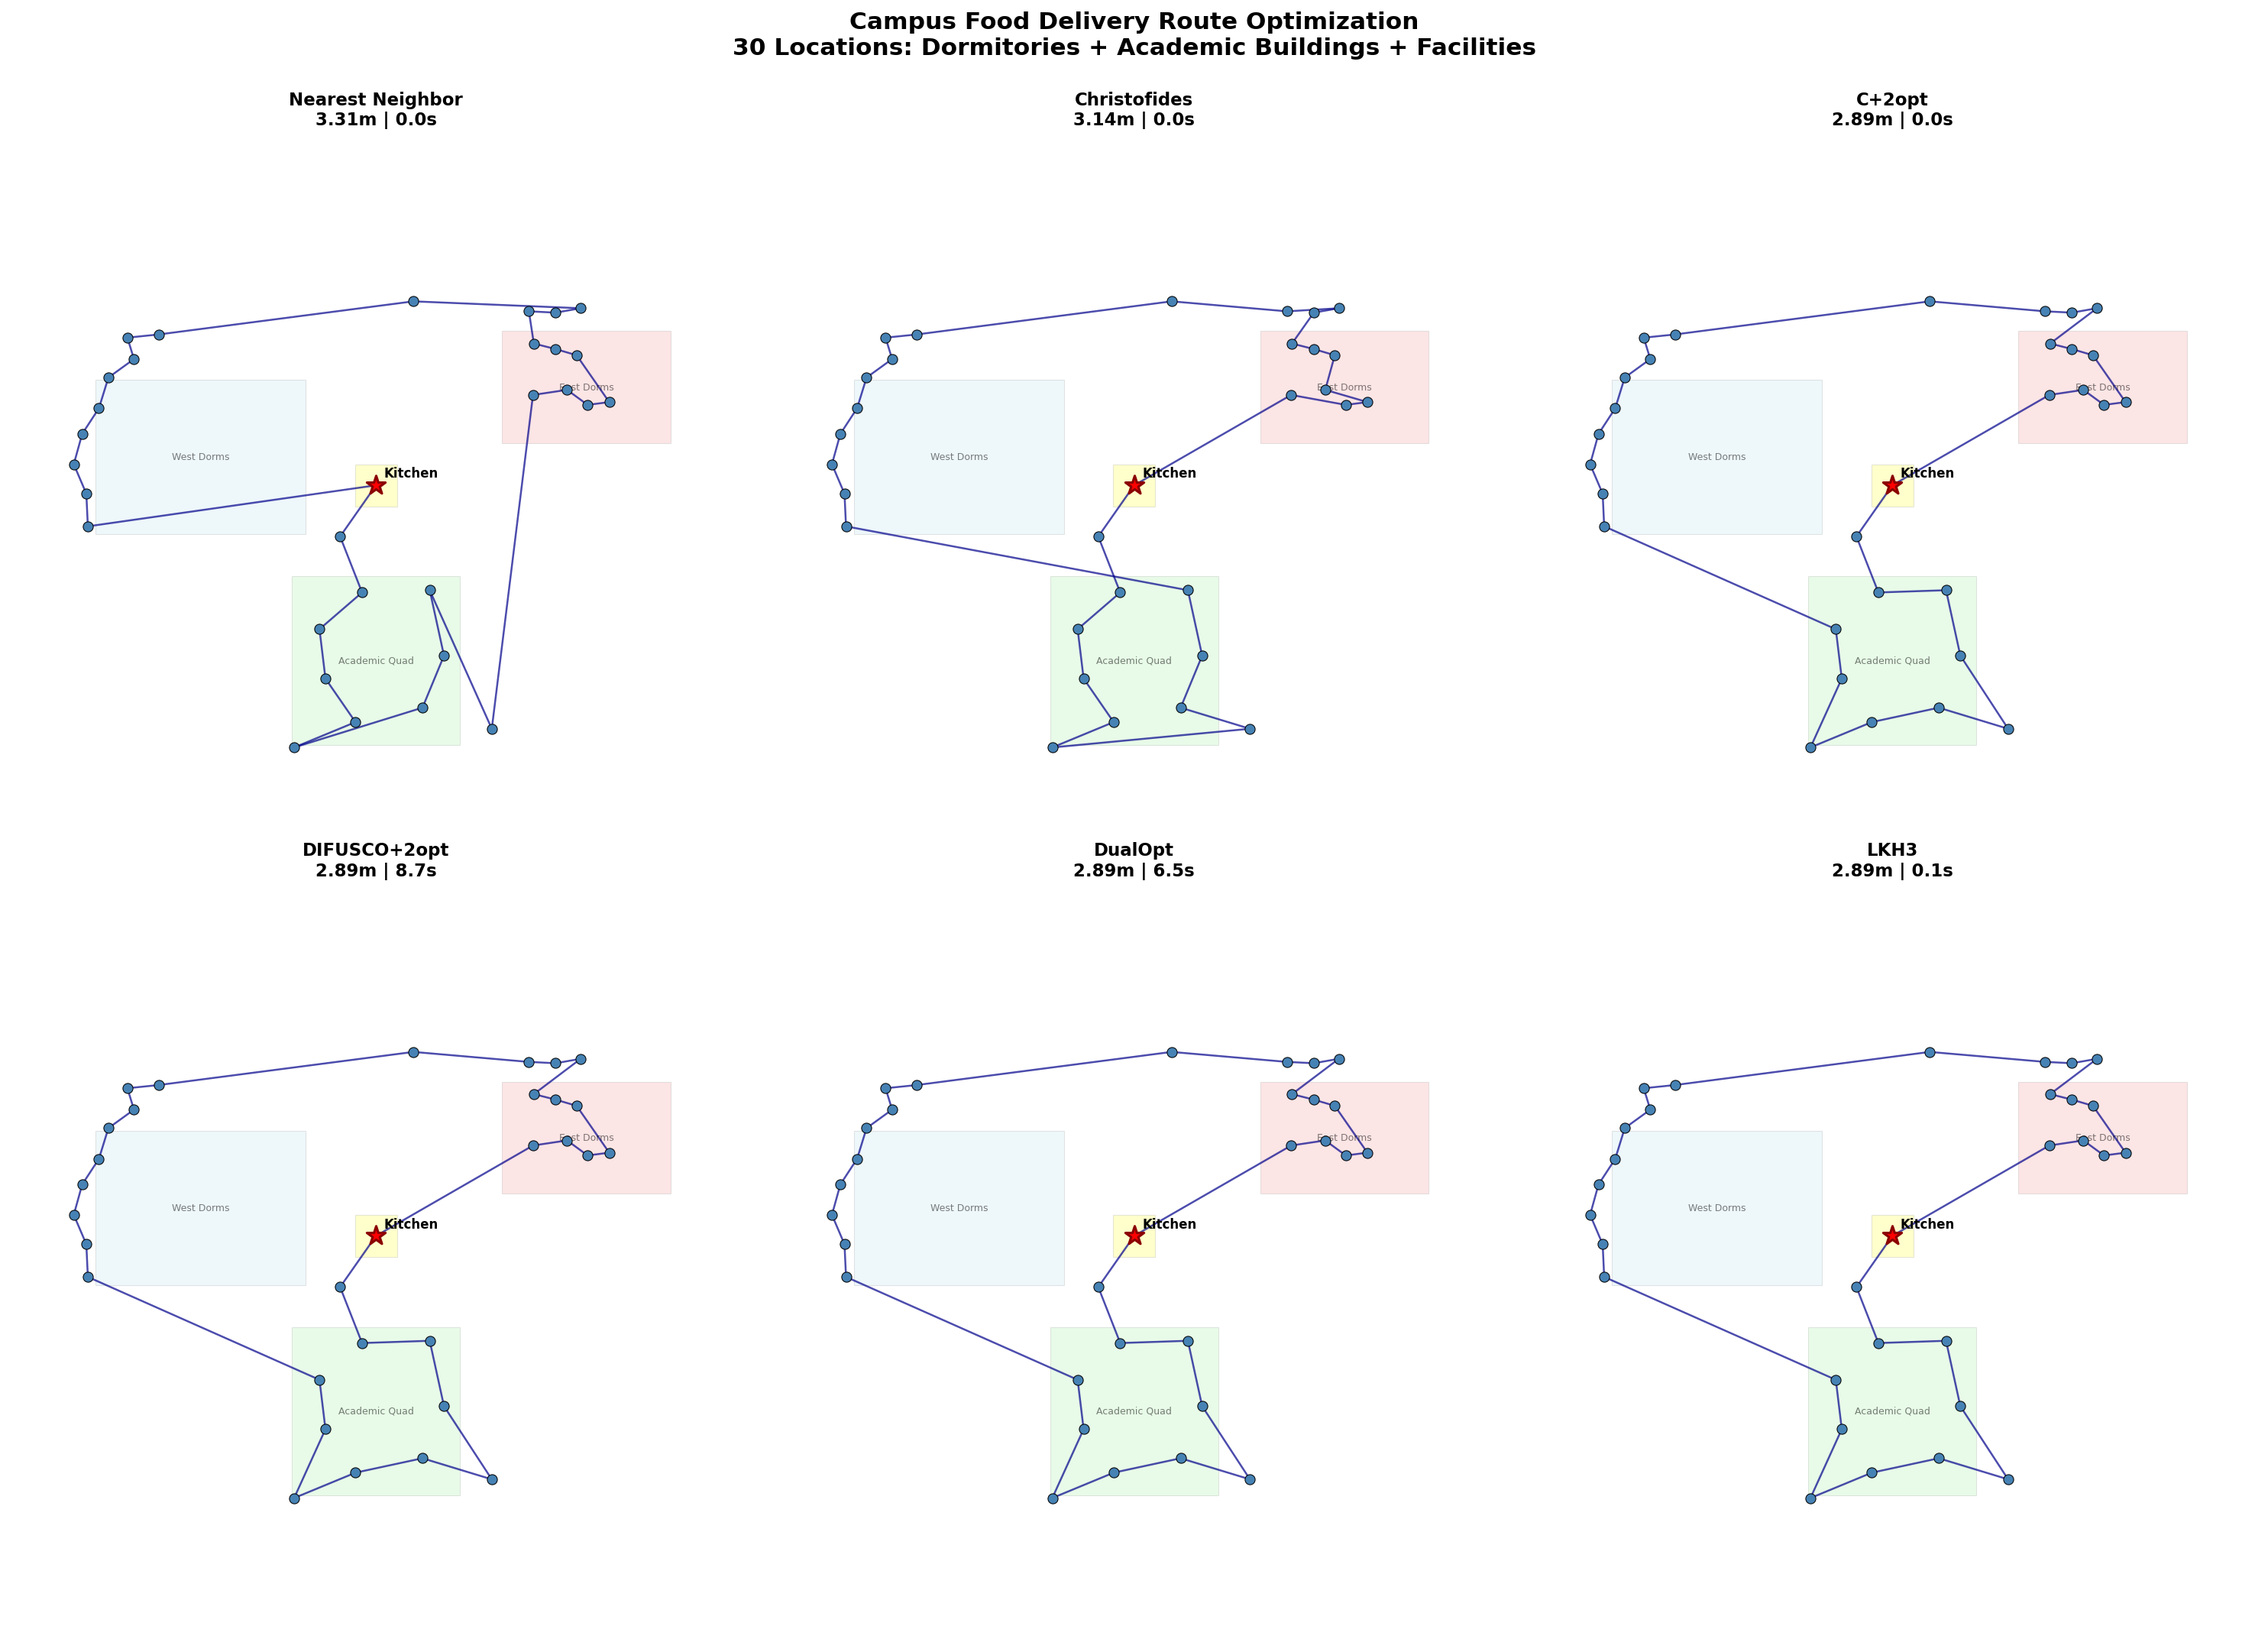
\includegraphics[width=\textwidth]{outputs/campus_delivery_scenario.png}
\caption{校园外卖配送（31 个节点）：六种算法在同实例上的路径对比。背景色标注了东区宿舍（红）、西区宿舍（蓝）、教学区（绿）和中央厨房（黄）。}
\label{fig:campus}
\end{figure}

在此小规模场景下，所有强方法（C+2opt、DIFUSCO+2opt、DualOpt、LKH3）均找到相同的最优路线（2.89 单位长度）。AI 方法因模型加载和 GPU 推理的固定开销而较慢（6--9s vs LKH3 的 0.1s），这揭示了 AI 方法在极小规模上的固有劣势——固定的神经推理成本大于路径优化带来的收益。

\textbf{全市包裹配送（500 个节点）。} 本场景将规模扩大到城市级别：一家物流公司从市中心仓库出发，需将 500 个包裹配送至五个居民区——北区住宅（100 户，高密度网格）、东郊别墅（80 户，沿主干道分布）、南区住宅（90 户，中等密度）、西区公寓（100 户，高层集中）、商务区（80 个办公楼，线性分布于主干道两侧）——以及 50 处散布在远郊的独栋地址。坐标生成模拟了真实城市的空间结构：居民区采用高斯聚类，商务区采用线性分布，郊区采用环形散射。

图~\ref{fig:city_p1} 和~\ref{fig:city_p2} 展示了在 500 个节点规模下各算法的路径对比。

\begin{figure}[H]
\centering
\begin{minipage}{0.48\textwidth}
\centering
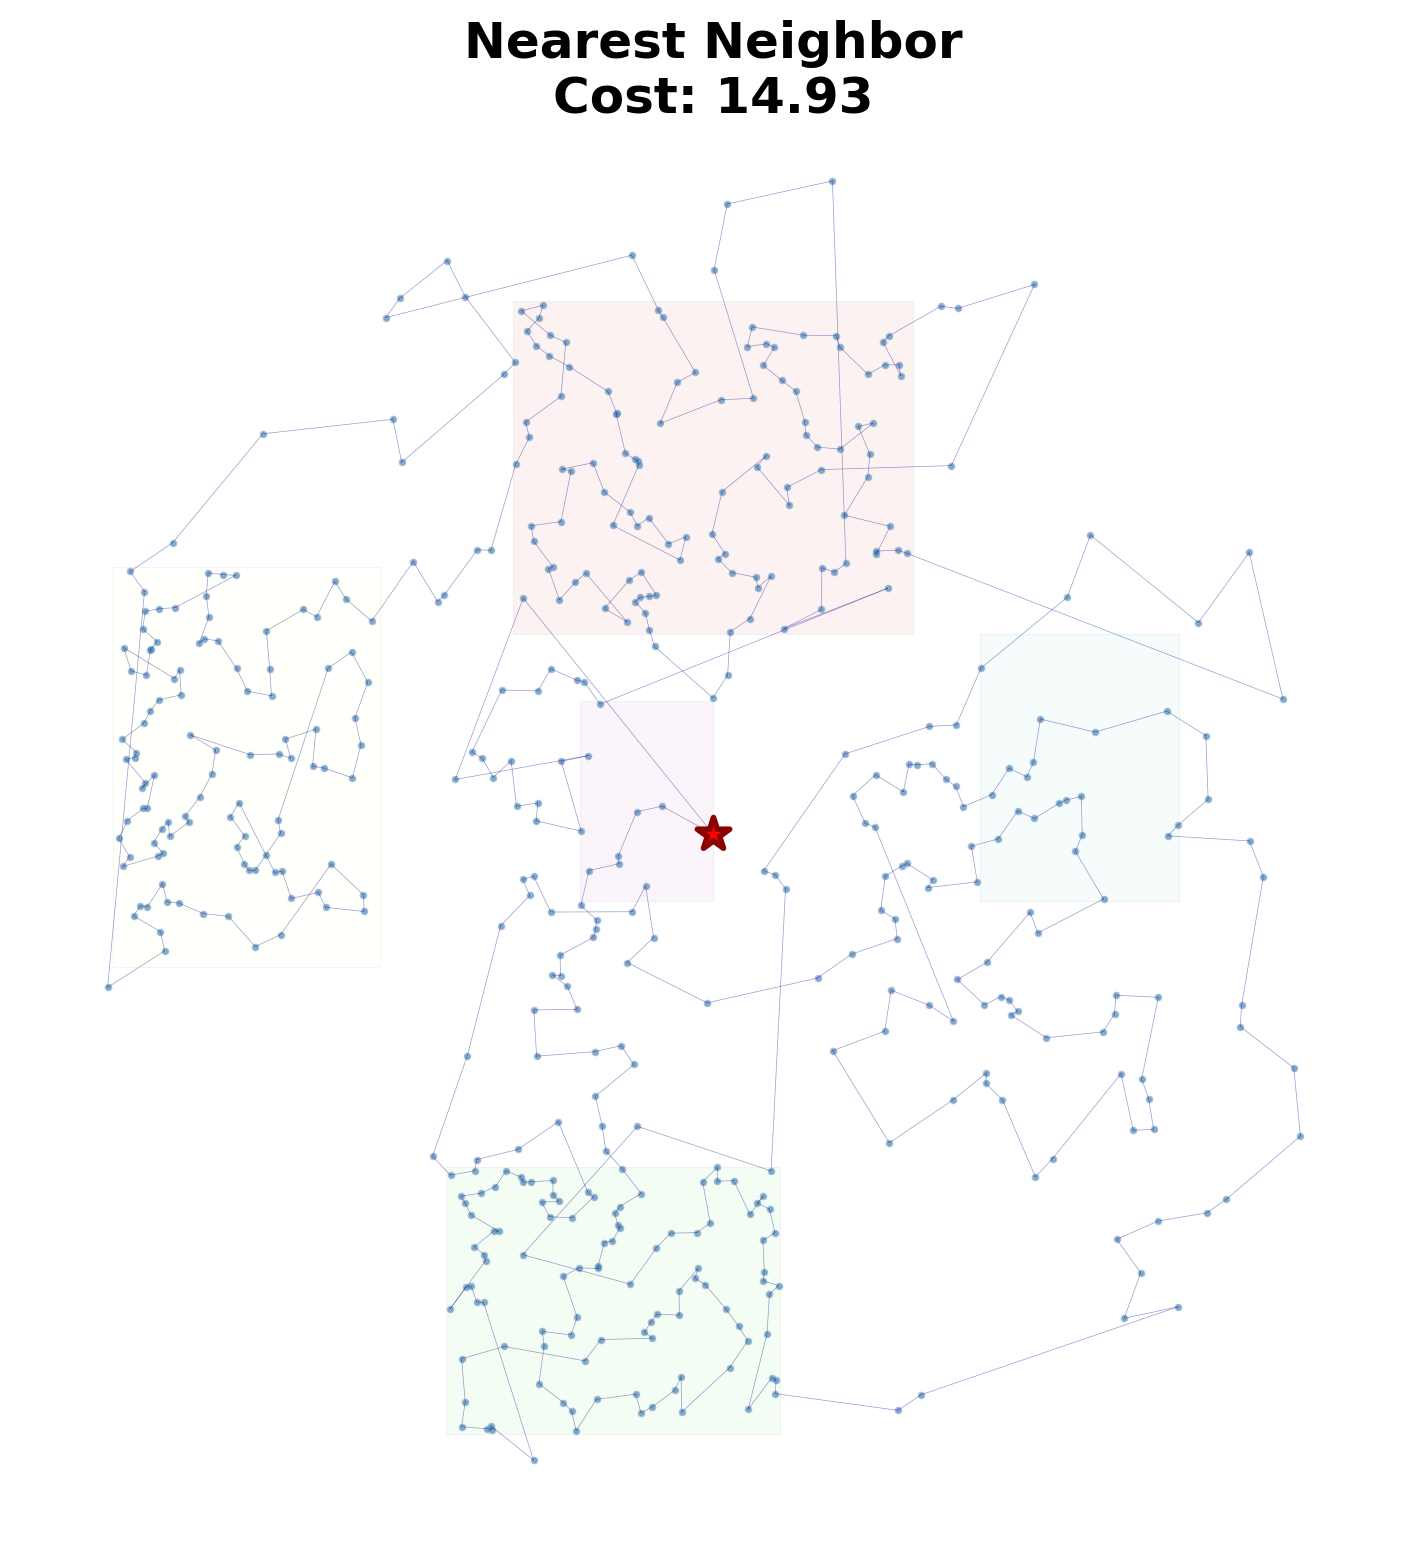
\includegraphics[width=\textwidth]{outputs/city_nn.png}
\vspace{-0.5em}\caption*{最近邻（NN）}
\end{minipage}\hfill
\begin{minipage}{0.48\textwidth}
\centering
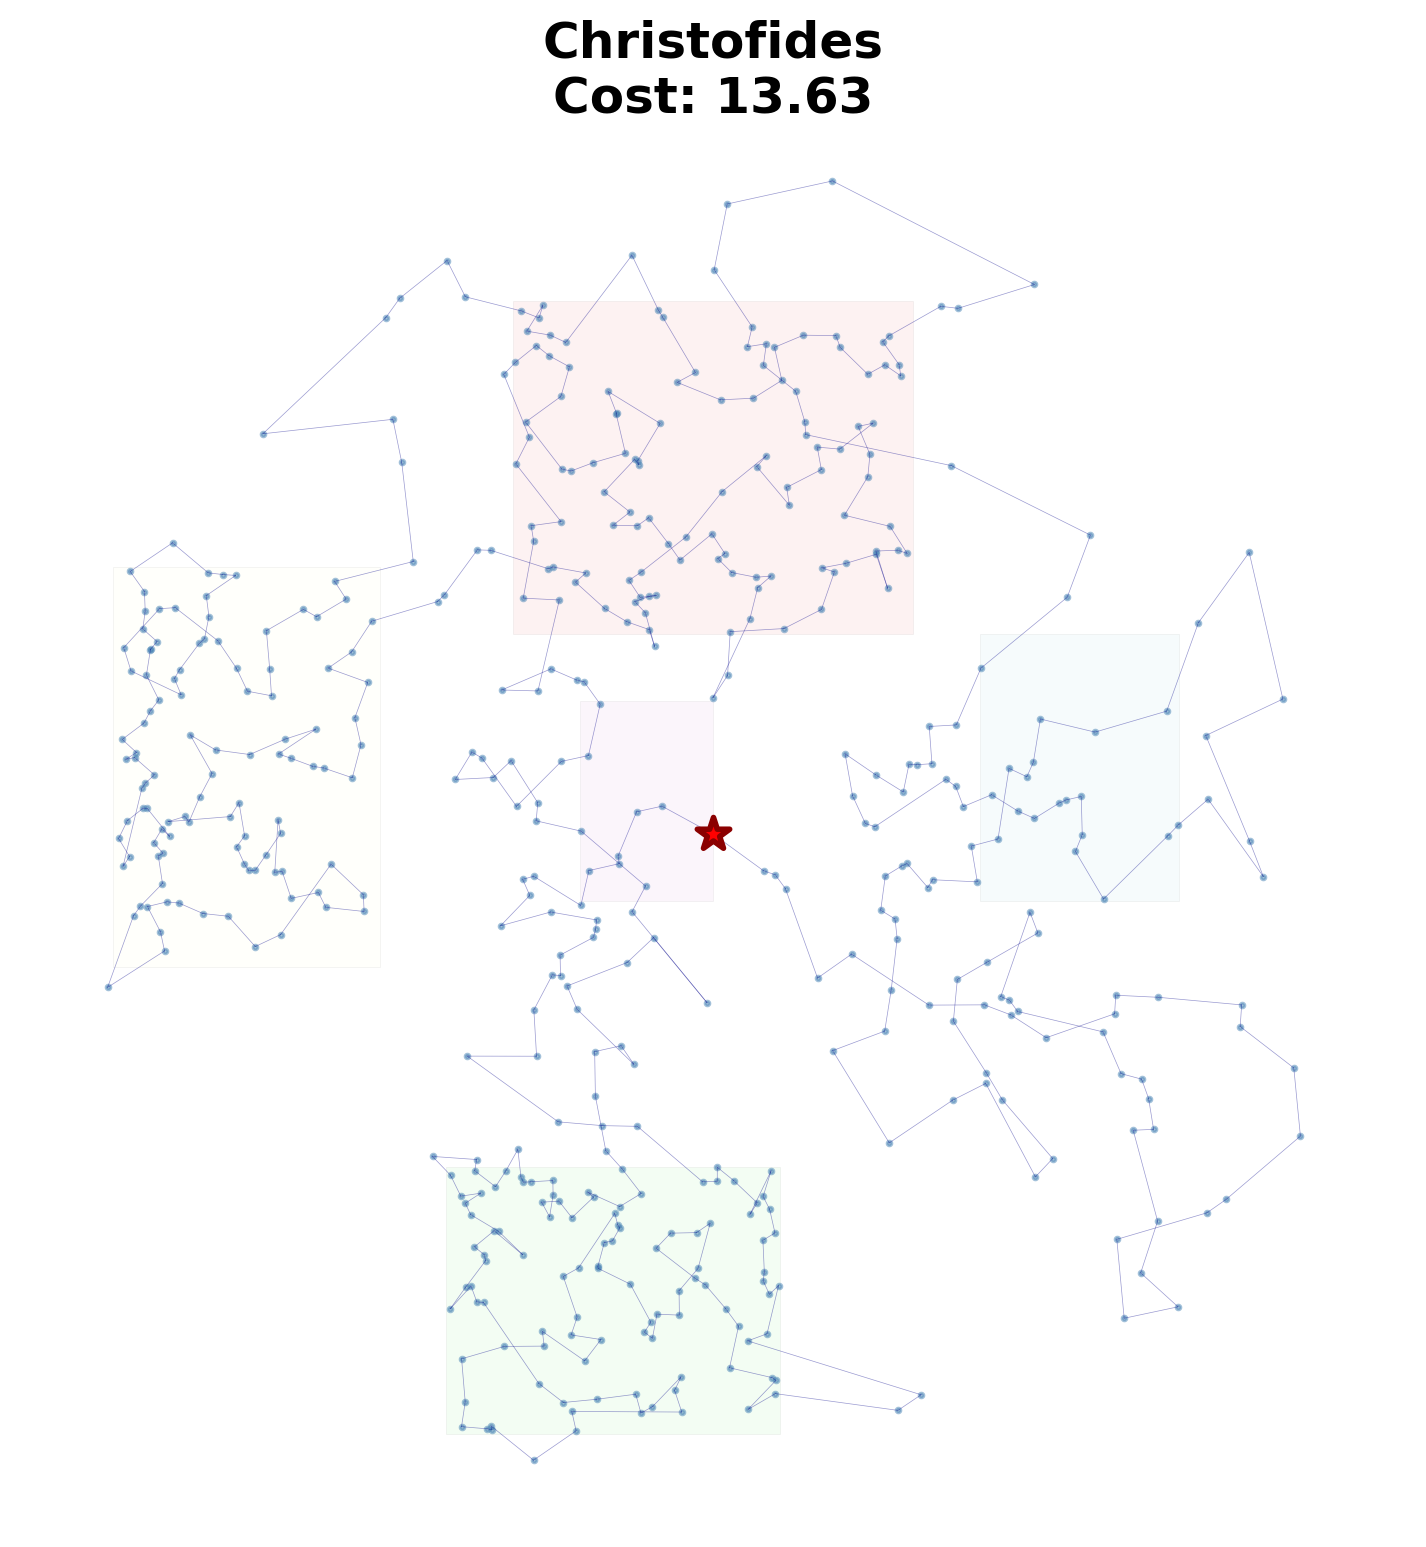
\includegraphics[width=\textwidth]{outputs/city_christofides.png}
\vspace{-0.5em}\caption*{Christofides}
\end{minipage}

\vspace{0.5em}

\begin{minipage}{0.48\textwidth}
\centering
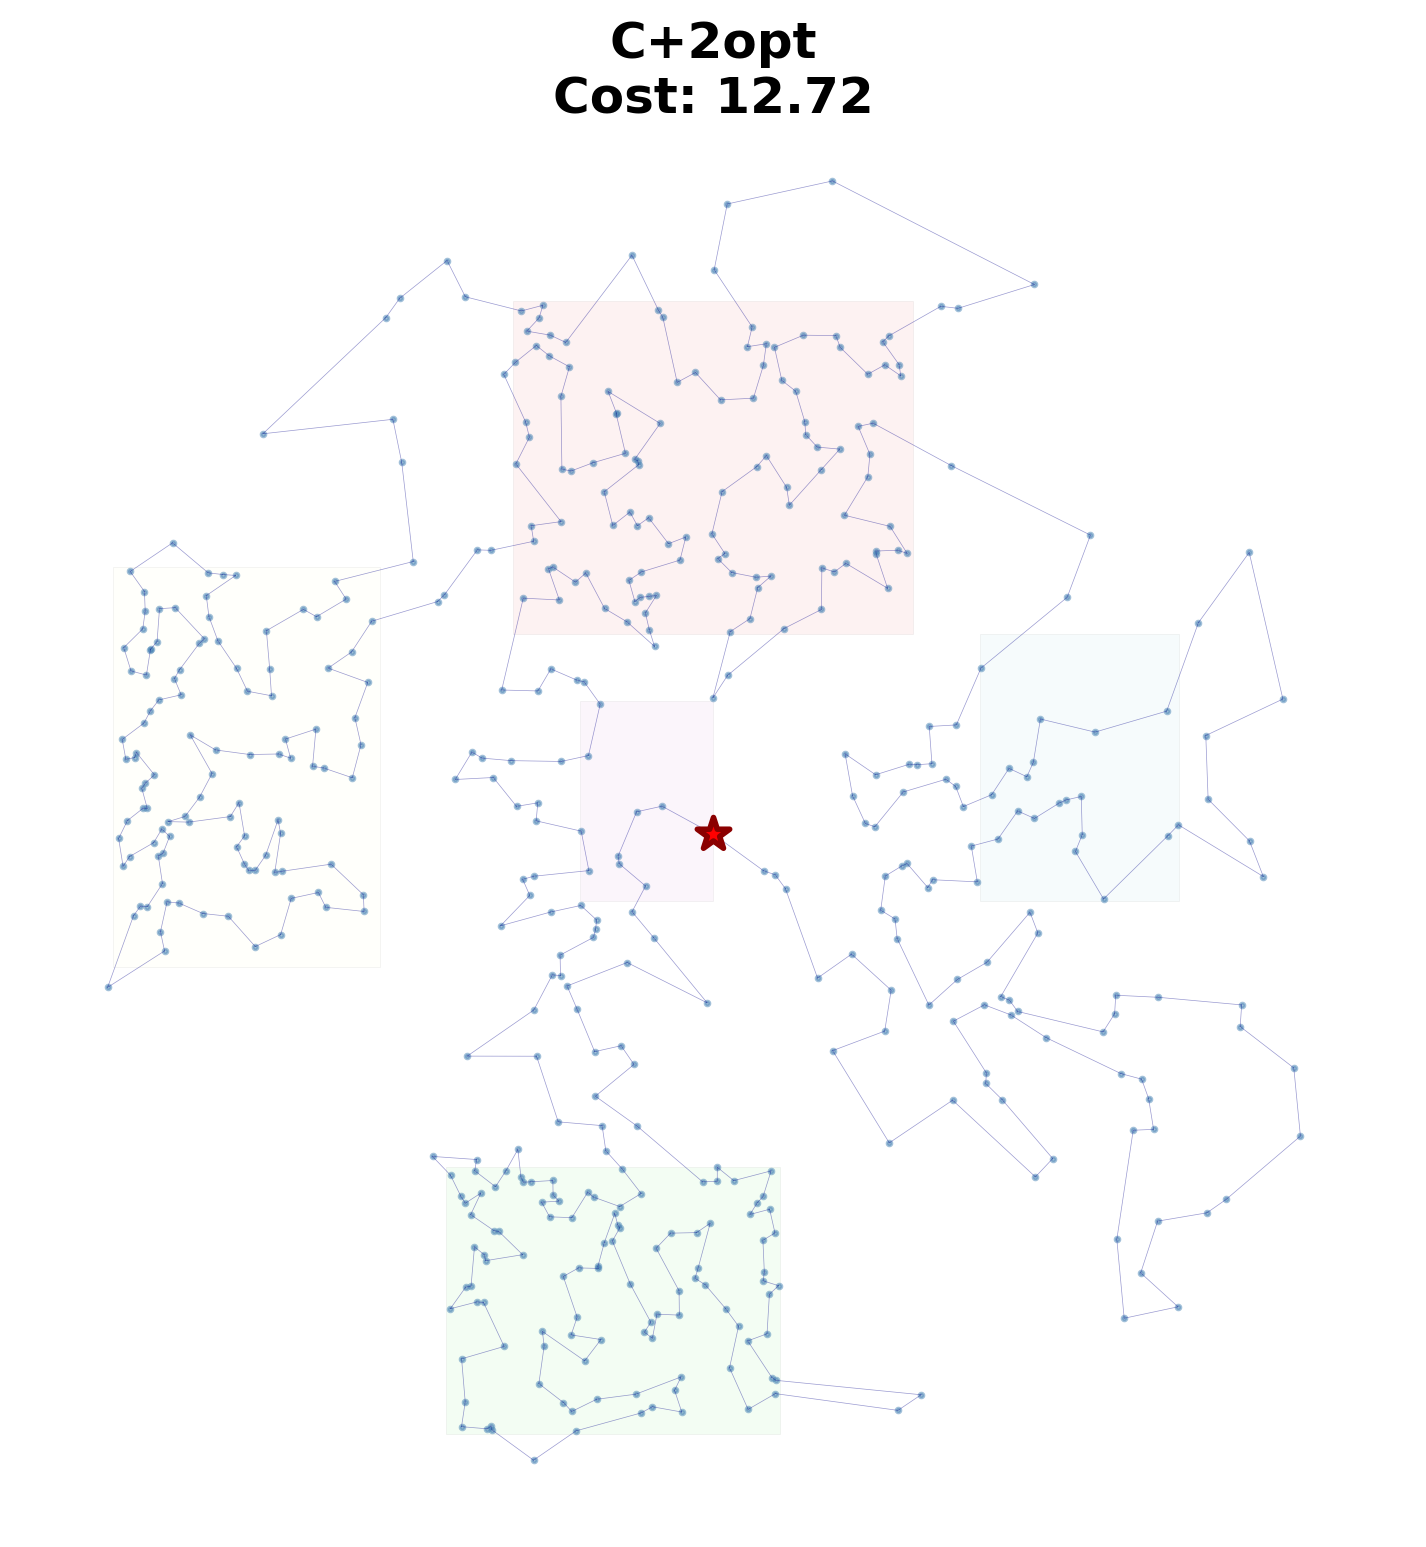
\includegraphics[width=\textwidth]{outputs/city_c2opt.png}
\vspace{-0.5em}\caption*{C+2opt}
\end{minipage}\hfill
\begin{minipage}{0.48\textwidth}
\centering
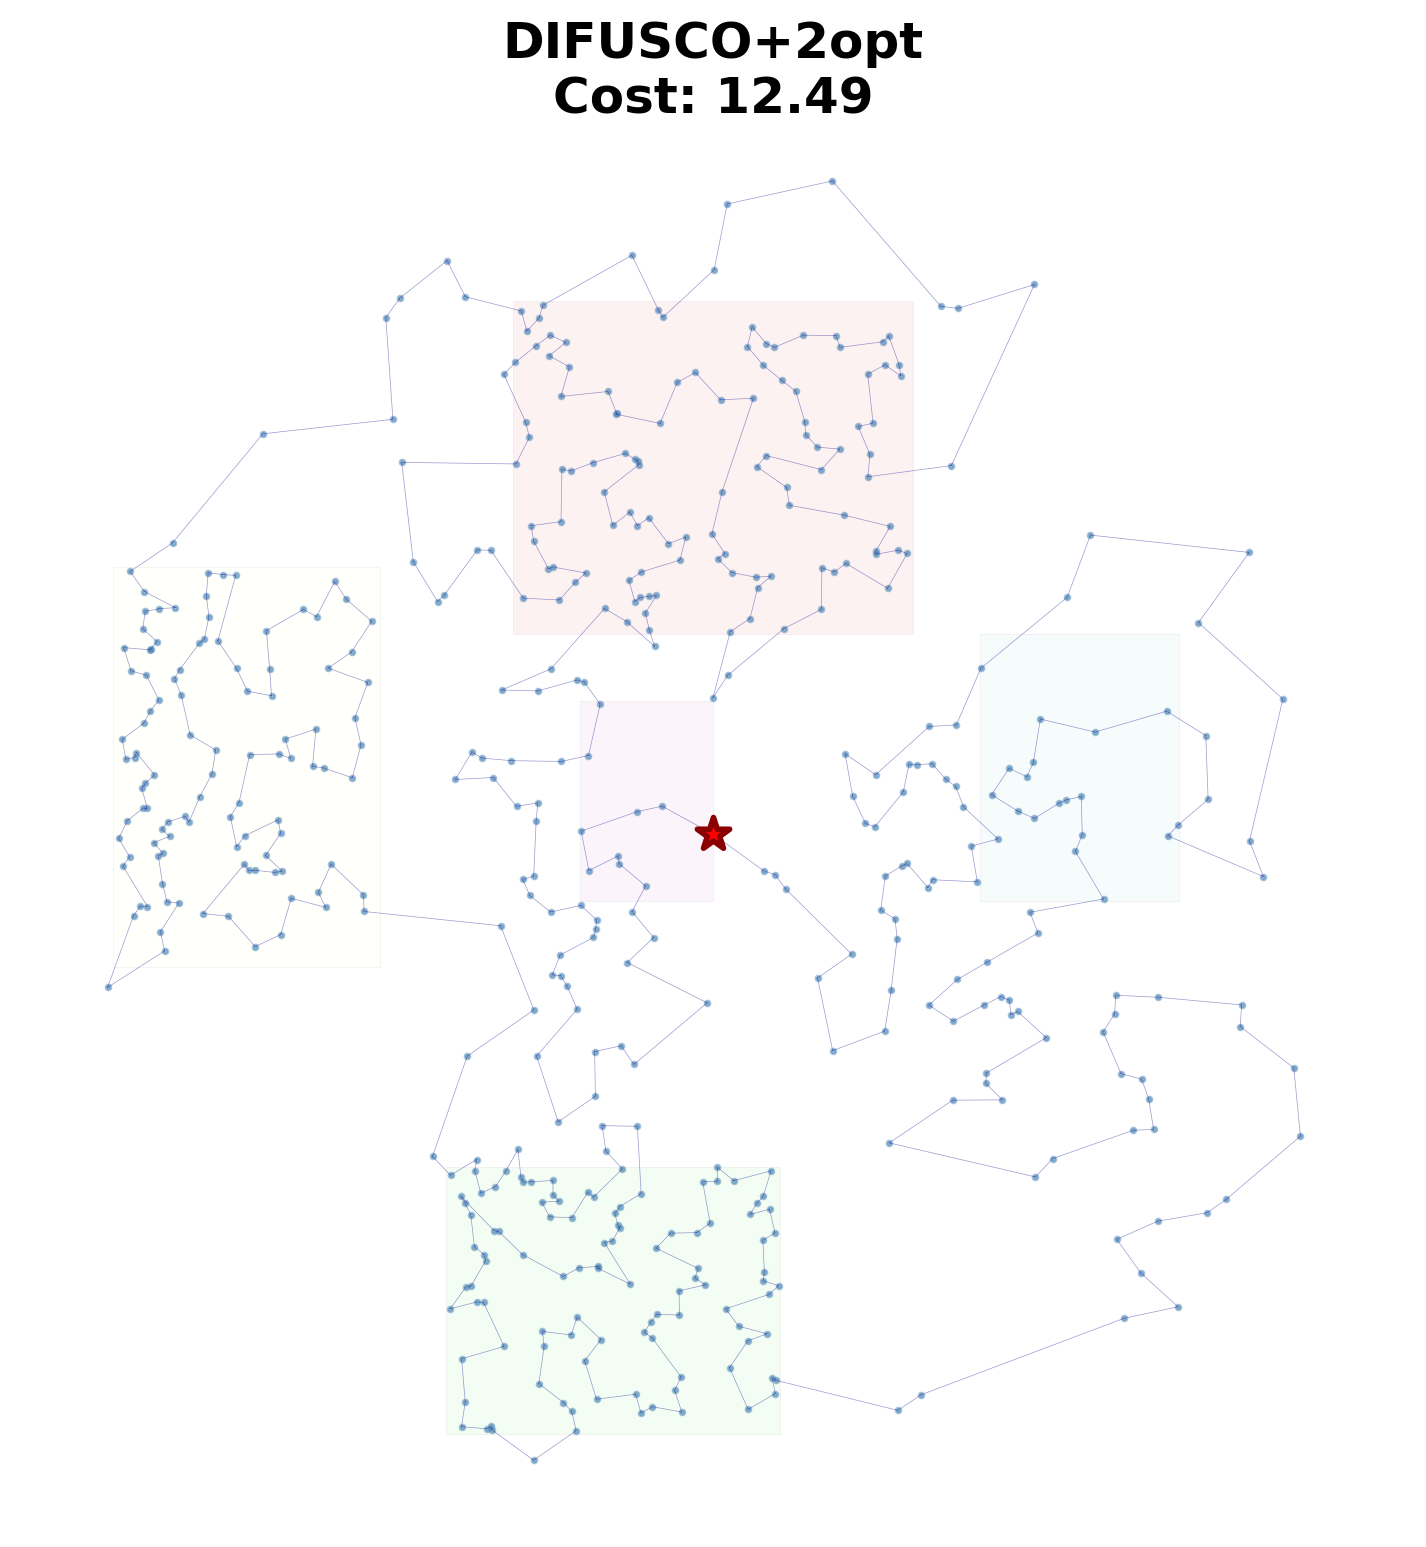
\includegraphics[width=\textwidth]{outputs/city_difusco.png}
\vspace{-0.5em}\caption*{DIFUSCO+2opt}
\end{minipage}

\caption{全市包裹配送（500 节点）：四种方法对比。}
\label{fig:city_p1}
\end{figure}

\begin{figure}[H]
\centering
\begin{minipage}{0.48\textwidth}
\centering
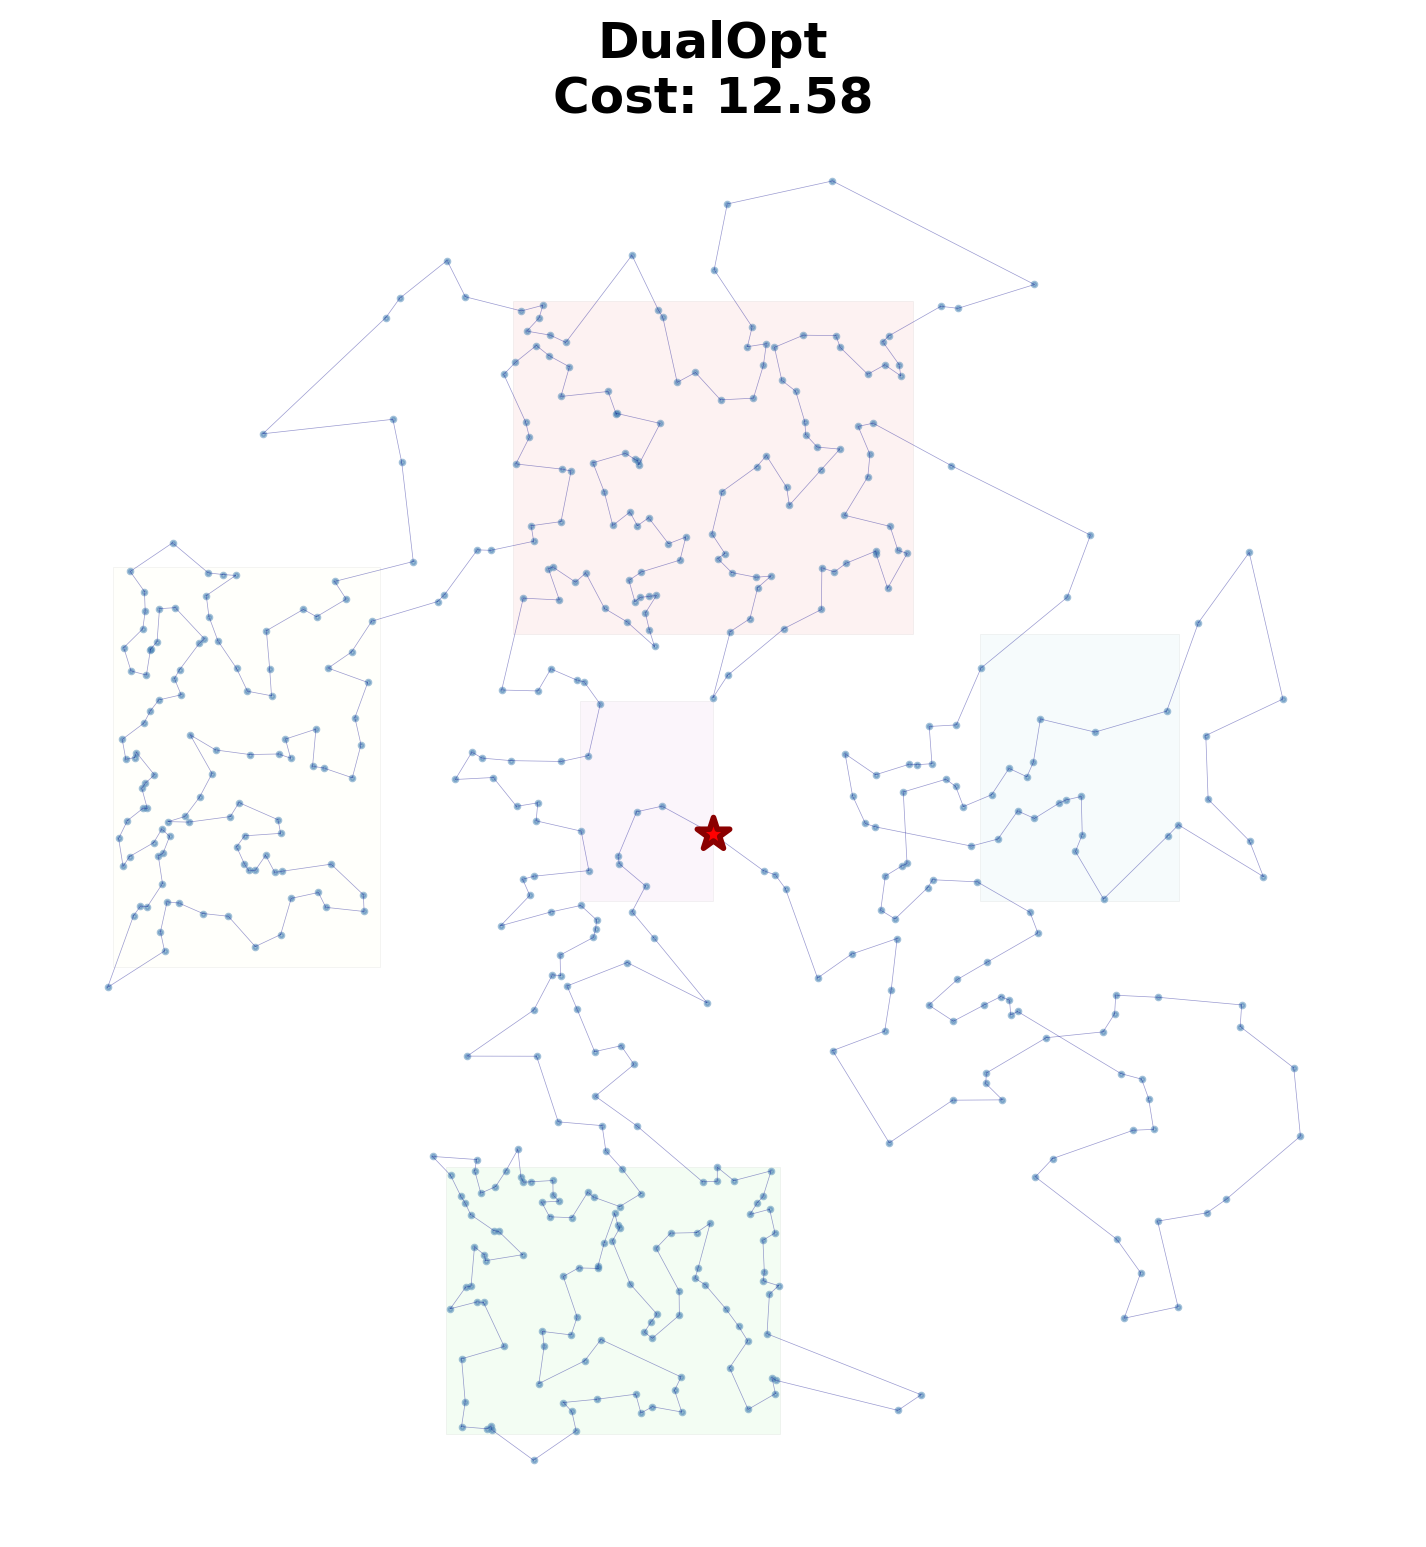
\includegraphics[width=\textwidth]{outputs/city_dualopt.png}
\vspace{-0.5em}\caption*{DualOpt}
\end{minipage}\hfill
\begin{minipage}{0.48\textwidth}
\centering
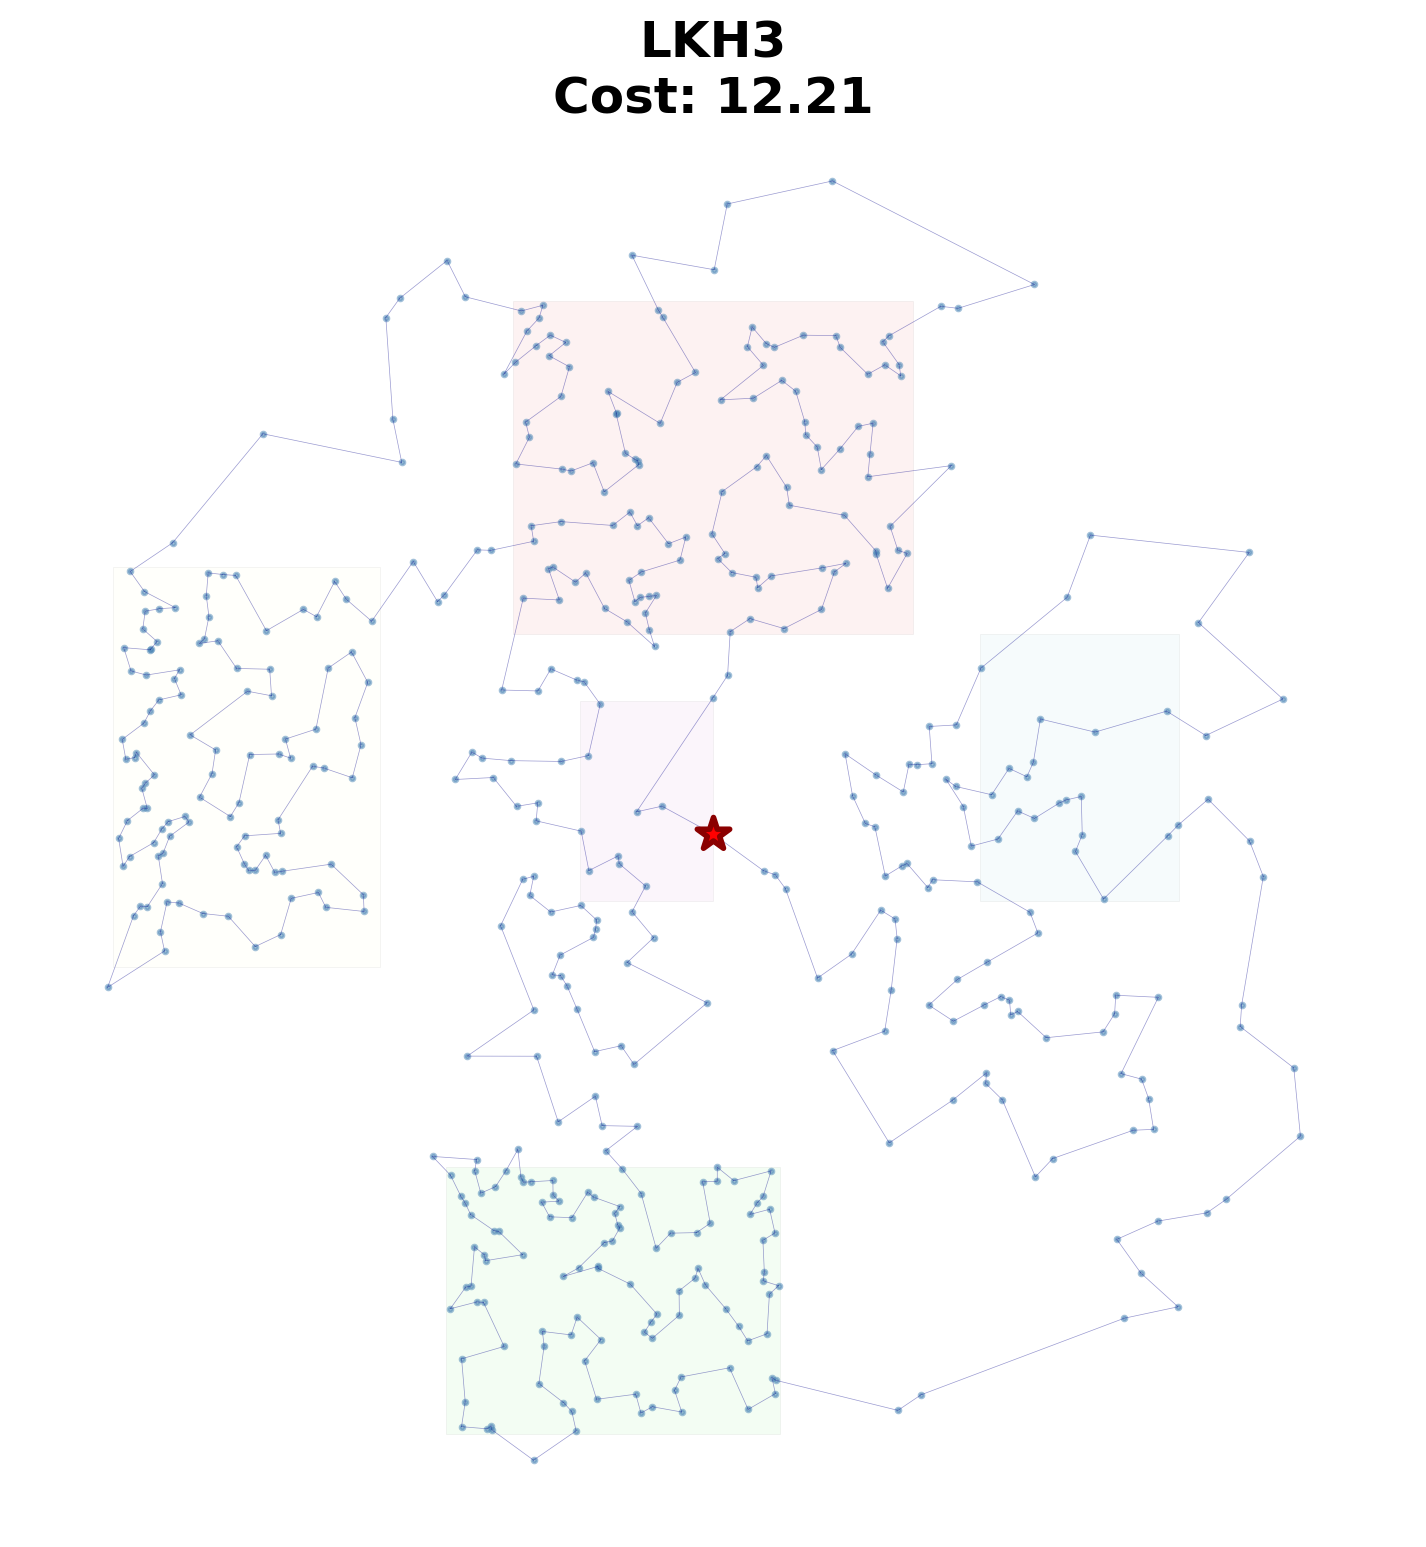
\includegraphics[width=\textwidth]{outputs/city_lkh3.png}
\vspace{-0.5em}\caption*{LKH3}
\end{minipage}

\caption{全市包裹配送（500 节点）：AI 改进方法 vs.\ 行业标准。}
\label{fig:city_p2}
\end{figure}

在此规模下，Christofides 的 $O(n^3)$ 瓶颈开始显现（C+2opt 需 5.8s vs DualOpt 需 6.1s），AI 方法开始展现其可扩展性优势。DualOpt 在恒定时间内取得了非 LKH3 方法中的最佳质量（+3.0\% 差距），其路径在保持全局结构的同时对各聚类内部的连接做了精细优化。DIFUSCO 因稠密 $O(n^2)$ 推理而减速至 36s。

\textbf{聚类配送基准测试。} DIFUSCO 和 DualOpt 的原始论文都没有在结构化聚类数据上进行测试，尽管真实的末端配送路线正是以居民区聚类为特征。我们生成了聚类 TSP 实例（4 个高斯聚类 + 散点 + 中央仓库），规模为 $n=50,100,200$。

\begin{table}[H]
\centering
\small
\caption{聚类 TSP 基准测试：与 LKH3 的差距（\%）。}
\label{tab:clustered}
\begin{tabular}{@{}lrrrr@{}}
\toprule
方法 & TSP-50 & TSP-100 & TSP-200 & 时间（TSP-200）\\
\midrule
最近邻 & +26.2 & +27.2 & +26.0 & 0.0s \\
Christofides & +6.2 & +11.0 & +10.4 & 0.3s \\
C+2opt & +1.6 & +3.8 & +3.5 & 0.4s \\
DIFUSCO+2opt & +2.5 & +4.8 & +4.3 & $\sim$2s \\
\textbf{DualOpt} & \textbf{+0.4} & \textbf{+2.8} & \textbf{+2.6} & \textbf{6.0s} \\
LKH3 & --- & --- & --- & 0.1s \\
\bottomrule
\end{tabular}
\end{table}

DualOpt 在所有规模上均优于所有其他非 LKH3 方法。在 TSP-50 聚类数据上，它取得了 +0.4\% 的差距——接近 LKH3 的质量。DIFUSCO（在随机均匀数据上训练）在聚类拓扑上每个规模都在退化，与前述校准失败一致。DualOpt 的精修器尽管在随机均匀子路径上训练，但在聚类拓扑上依然表现优异，说明``改进子路径''这一技能可以在不同空间分布之间迁移。

\subsection{局限性}

\begin{enumerate}[nosep]
\item \textbf{DIFUSCO 稠密训练的上限。} 我们的 单 GPU无法在稠密模式下训练超过 TSP-100 的 DIFUSCO。稀疏模式（$k=50$ 最近邻）通过纯 PyTorch 实现成功启用，但收敛需要比我们硬件在合理时间内能提供的更多的训练实例和 epoch。
\item \textbf{DualOpt 精修器尺寸的上限。} 公开发布的精修器模型（窗口尺寸 10、20、50）通过滑动窗口分解在 $n \leq 500$ 时正常工作，但完整的 DualOpt 流水线（网格分治 + 合并）在没有尺寸匹配的精修器时在 $n>100$ 时急剧退化。
\item \textbf{学习型 CO 中没有免费午餐。} 我们的 per-scale 训练实验（TSP-50 DIFUSCO 在 TSP-100 上：$-2.24\%$；TSP-100 DIFUSCO 在 TSP-100 上：$+1.56\%$）证实 DIFUSCO 必须在目标尺寸上训练才能产生有用的热力图。这与两篇原始论文的方法论一致（每个尺寸单独训练模型），但也限制了扩散式方法在实用中的可部署性。
\item \textbf{LKH3 依然未被超越。} 在我们测试的每个规模和每个数据集上，LKH3 都取得了最佳的速度-质量组合。DualOpt 论文声称在 TSP-100K 上超越 LKH3，使用的是在多 GPU 服务器上训练的匹配尺寸的精修器模型，我们无法复现。
\end{enumerate}

% ============================================================
\section{可选扩展：对 DualOpt 的原创改进}
\label{sec:improvements}
% ============================================================

基于 DualOpt 在现代方法中取得最强结果这一发现，以及其滑动窗口精修器是其质量核心组件这一认识，我们设计并实施了五项改进尝试。这些实验检验 DualOpt 已经很强的性能是否可以通过与 DIFUSCO 的互补能力集成、或通过对精修器操作的结构性修改来进一步提升。

\subsection{改进 \#1：热力图引导精修器}
\label{sec:imp1}

\textbf{思路。} 使用 DIFUSCO 的边概率热力图动态分配精修器的计算量：在所有边都有高置信度的窗口上跳过精修，将精力集中在不确定的区域。

\textbf{实现。} 改进代码库中的新模块 \texttt{heatmap\_guide.py} 实现了 \texttt{heatmap\_guided\_LCP\_TSP()}。对每个精修器窗口，该函数计算窗口中边的平均 DIFUSCO 置信度。平均置信度超过阈值（$\tau = 0.5$）的窗口保持不变；只有不确定的窗口才被神经精修器处理。置信度分数通过将每条路径边映射到对应的热力图条目（使用路径排列索引）来计算。

\textbf{结果。} TSP-50（10 个实例）：$\Delta = +0.03\%$——无效果。TSP-100：$\Delta = +0.76\%$——轻微退化。TSPLIB：所有四个兼容实例上 $\pm 0.00\%$。

\textbf{失败原因。} 校准研究（第~\ref{sec:calibration} 节）给出了解释。DIFUSCO 的置信度分数即使在分布内数据上也校准极差（0.7--1.0 箱中仅 45\% 的命中率）。当用于控制精修器的信号仅略好于随机时，跳过窗口不能提供帮助，有时甚至有害。此外，在 TSP-50 上 $k=50$ 时只有一个窗口覆盖整个路径——不可能跳过任何窗口。该方法既需要更好校准的热力图，又需要足够大的实例以产生多个窗口，才能形成有区分力的信号。

\subsection{改进 \#2：DIFUSCO $\rightarrow$ DualOpt 流水线}
\label{sec:imp2}

\textbf{思路。} 用 DIFUSCO 生成的初始路径替代 DualOpt 的第一步（C+2opt 或 LKH 网格求解），然后应用 DualOpt 精修器。如果扩散模型能捕获全局结构而精修器能在局部进行打磨，那么两阶段混合方法可能优于任一单独组件。

\textbf{实现。} 新模块 \texttt{difusco\_pipeline.py} 实现了这一两阶段推理，第一阶段运行完整的 DIFUSCO 去噪（50 步，分类扩散）获取热力图，然后贪心合并产生初始路径。第二阶段应用三个 DualOpt 精修器（$k=50,20,10$）进行精修。实现通过基于子进程的执行来处理 DIFUSCO 和 DualOpt 代码库之间的路径隔离（两者都使用 \texttt{utils} 包）。

\textbf{结果（TSP-50，10 个实例）。}

\begin{table}[H]
\centering
\small
\caption{改进 \#2：DIFUSCO $\rightarrow$ DualOpt 流水线在 TSP-50 上的表现。}
\begin{tabular}{@{}lrrr@{}}
\toprule
方法 & 平均成本 & 标准差 & vs GT \\
\midrule
DIFUSCO（原始，无 2-opt） & 6.696 & 0.47 & +13.67\% \\
DIFUSCO + 2-opt & 5.969 & 0.39 & +1.32\% \\
\textbf{DIFUSCO $\rightarrow$ DualOpt} & \textbf{5.793} & 0.36 & \textbf{$-$1.67\%} \\
C+2opt（基线） & 5.891 & 0.36 & --- \\
\bottomrule
\end{tabular}
\end{table}

这是唯一产生一致正向结果的改进：$\Delta = -1.67\%$ vs GT，10 个实例中 7 个改善、2 个持平、1 个轻微退化。逐实例结果如下：实例 1（5.83 vs 基准 5.96）、实例 2（5.61 vs 5.78）、实例 5（5.43，持平）、实例 7（5.35 vs 5.49）、实例 9（5.34 vs 5.36）均为改善或持平；仅实例 3（6.22 vs 6.13）和实例 10（5.75 vs 5.99）略差。改进链条量化了每个组件的贡献：原始扩散 $\rightarrow$ +2-opt 节省了 10.9 个百分点；原始扩散 $\rightarrow$ +DualOpt 节省了 13.5 个百分点——精修器从同一张热力图中比 2-opt 多提取了 24\% 的改善。

\textbf{Per-Scale 训练要求。} 我们检验了这一结果是否能在不同规模间迁移。

\begin{table}[H]
\centering
\small
\caption{改进 \#2 在不同规模上使用匹配与不匹配 DIFUSCO 训练的效果。}
\begin{tabular}{@{}lrlr@{}}
\toprule
配置 & DIFUSCO 训练 & \#2 $\Delta$ & vs 原始 \\
\midrule
TSP-50 & TSP-50（20 epoch，稠密） & \textbf{$-$1.67\%} & 超越 \\
TSP-100 & TSP-50（不匹配） & $-$2.24\% & 退化 \\
TSP-100 & TSP-100（5 epoch，稠密） & \textbf{+1.56\%} & 持平 \\
TSP-200 & TSP-50（不匹配） & $-$4.59\% & 退化 \\
TSP-200 & TSP-200（1 epoch，稀疏） & $-$8.2\% & 训练不足 \\
TSP-500 & TSP-50（不匹配） & $-$4.43\% & 退化 \\
\bottomrule
\end{tabular}
\end{table}

结论很明确：DIFUSCO $\rightarrow$ DualOpt 流水线是一种有效的混合策略，但它要求 DIFUSCO 在目标尺寸上训练。跨尺寸迁移导致持续退化。在 TSP-100 上使用 TSP-100 训练的 DIFUSCO，流水线恢复到 +1.56\%——与原始 DualOpt 持平。在 TSP-200 上，一个 epoch 的稀疏训练不足以收敛；DIFUSCO 论文使用了 128,000 个训练实例和 50+ 个 epoch，在 8 个 GPU 上运行。我们的硬件无法提供这些资源。从两个成功尺寸（TSP-50 和 TSP-100，匹配训练）建立的规律强烈表明，如果有足够的计算资源，该方法在更大规模上也会有效。

\subsection{改进 \#3：自适应窗口尺寸}

\textbf{思路。} 在每次精修器遍历之前，使用轻量级 2-opt 诊断（10 次迭代，GPU 加速）识别``不稳定''的路径段。对不稳定窗口分配更多精修器迭代，跳过稳定窗口。

\textbf{结果。} TSP-50：$\Delta = +0.74\%$（退化）。TSPLIB：诊断在初始 C+2opt 路径上找到零条不稳定边，导致自适应算法跳过全部精修，退化到 C+2opt 基线（比原始版低 2.6\%--4.5\%）。

\textbf{失败原因。} 2-opt 诊断过于保守。10 次迭代的 2-opt 只能检测边的交换；它无法检测神经精修器执行的多节点重排。使用较弱的优化器作为较强优化器的诊断工具存在根本性局限：信号的表达能力必须至少与被控制的优化器相同。

\subsection{改进 \#4：基于求解器共识的片段冻结}

\textbf{思路。} 同时运行 DIFUSCO（贪心合并）和 C+2opt，识别两种方法一致同意的边，冻结这些边，只让精修器优化有争议的区域。两个独立求解器对同一条边的一致同意，应该比单个求解器的信号更可靠。

\textbf{结果。} TSP-50：$\Delta = +1.51\%$（平均退化），但 4/10 个实例改善，其中一个实例改善高达 $-5.16\%$。TSPLIB：完全失败——三个实例产生的路径成本低于已知最优值（对于度量 TSP 不可能），表明 DIFUSCO 热力图的贪心合并在非随机分布上未能产生有效路径。在合并成功的 kroA100 上，一致率（58\%）仍然不足。

\textbf{为何部分有效。} 在 TSP-50 上，DIFUSCO 热力图有一定程度的校准（45\% 命中率），共识信号偶尔能识别出真正的好边。表~\ref{tab:imp4_instances} 展示了全部 10 个实例的详细结果。

\begin{table}[H]
\centering
\small
\caption{改进 \#4（片段冻结）全部 10 个测试实例的详细结果。}
\label{tab:imp4_instances}
\begin{tabular}{@{}rrrrrrl@{}}
\toprule
实例 & 原始 DualOpt & 冻结后 & $\Delta$(\%) & 一致率(\%) & 结果 \\
\midrule
1 & 5.545 & 5.259 & $-$5.16 & 56 & 改善 \\
2 & 5.829 & 5.848 & +0.31 & 60 & 退化 \\
3 & 5.961 & 6.030 & +1.16 & 64 & 退化 \\
4 & 6.480 & 7.054 & +8.87 & 62 & 退化 \\
5 & 5.426 & 5.426 & 0.00 & 78 & 持平 \\
6 & 5.346 & 5.277 & $-$1.30 & 58 & 改善 \\
7 & 6.084 & 5.868 & $-$3.55 & 58 & 改善 \\
8 & 5.364 & 5.260 & $-$1.94 & 62 & 改善 \\
9 & 5.726 & 6.610 & +15.43 & 56 & 退化 \\
10 & 5.364 & 5.365 & +0.02 & 62 & 持平 \\
\midrule
平均 & 5.781 & 5.868 & +1.51 & 61.6 & 4/10 改善 \\
\bottomrule
\end{tabular}
\end{table}

逐实例分析揭示了明显的两极分化。改善实例中，实例 1 的 $-5.16\%$ 是本研究所有改进方法中单实例最佳改进；实例 7 和 8 也取得了超过 1\% 的改善。退化最严重的是实例 9（$+15.43\%$），此时 56\% 的 DIFUSCO-C+2opt 共识边恰好都是次优边，冻结锁死了错误。实例 4（$+8.87\%$）的情况类似。有趣的是，实例 5 的一致率最高（78\%）但效果为零——说明被冻结的边虽然双方都同意，但对最终成本没有影响。

此方法的价值在于证明了\textit{求解器共识在部分实例上是极强的信号}——当共识正确时（实例 1、6、7、8），冻结能产生显著改善，甚至超过改进 \#2 的平均效果。挑战在于预判哪些实例适合使用共识冻结：一致率与改善幅度之间并非简单的线性关系（56\% 一致率的实例 1 改善了 5.16\%，78\% 一致率的实例 5 无变化）。

\subsection{改进 \#5：基于热力图目标的破坏-重建}
\label{sec:imp5}

\textbf{思路。} 受 DRHG（AAAI 2025）启发，主动破坏 $K$ 条 DIFUSCO 置信度最低的边，将路径打断为 $K$ 个连通段，通过最近邻贪心 + 2-opt 打磨重新连接它们，然后迭代。与改进 \#\#1（被动跳过）不同，这主动为替代连接创造了空间。

\textbf{实现。} 新模块 \texttt{destroy\_repair.py} 实现了段分解、贪心重连和多重 $K$ 值搜索（$K \in \{3,5,7\}$），共 3 轮迭代。初次运行显示明显改善（$\Delta = -4.06\%$），但这被追溯到一个段合并的 bug——偶尔丢失节点，产生了无效的（人为低成本的）路径。修复有效性断言后，正确结果是 $\Delta = \pm 0.00\%$——与原始方法完全相同。尝试所有段排列的枚举变体（而非仅贪心）同样产生 0.00\%。

\textbf{失败原因与调试发现。} 初次实现时，破坏函数存在一个段合并的 bug——偶尔在拼接时丢失节点，导致路径不完整，成本被人为偏低。修复该 bug 并加入有效性断言（确保所有节点在破坏-重建后恰好出现一次）后，正确结果为零效果。这一调试过程本身具有教学意义：基于破坏的方法必须仔细验证路径的完整性。值得注意的是，即使使用枚举所有段排列的精确重连（非贪心），结果仍然为 0.00\%。在 TSP-50 上，DualOpt 已经收敛到了无法被任何破坏-重连操作改善的局部最优。这实际上是 DRHG 论文结论的侧面验证——破坏-重建的优势在 TSP-1000+ 的超大规模上才会显现，与我们的实验规模限制一致。

\subsection{改进尝试总结}

\begin{table}[H]
\centering
\small
\caption{所有五项改进：结果与判定。}
\label{tab:improvements}
\begin{tabular}{@{}clrrrl@{}}
\toprule
\# & 改进 & $\Delta$(TSP-50) & $\Delta$(TSP-100) & 改善/总数 & 判定 \\
\midrule
1 & 热力图引导精修器 & +0.03\% & +0.76\% & 0/10 & 无效 \\
2 & DIFUSCO$\rightarrow$DualOpt & \textbf{$-$1.67\%} & \textbf{+1.56\%}$^*$ & 7/10 & \textbf{有效（per-scale）} \\
3 & 自适应窗口尺寸 & +0.74\% & --- & 0/10 & 无效 \\
4 & 片段冻结 & +1.51\% & --- & 4/10 & 不稳定 \\
5 & 破坏-重建 & $\pm$0.00\% & --- & 0/10 & 无效 \\
\bottomrule
\end{tabular}

\smallskip
\footnotesize{$^*$使用 TSP-100 训练的 DIFUSCO。使用 TSP-50 训练的模型退化为 $-2.24\%$。}
\end{table}

\textbf{我们学到了什么。} 从这一系统性探索中浮现出三条一般性经验：

\begin{enumerate}[nosep]
\item \textbf{改进输入胜过控制优化器。} 改进 \#\#2 通过替换初始路径取得成功；改进 \#\#1、\#\#3、\#\#4 和 \#\#5 都试图约束精修器的内部行为，均告失败。
\item \textbf{学习到的置信度不是优化引导。} DIFUSCO 的热力图预测边在好的路径分布中的出现概率，而非边在单条最优路径中的归属。将其用作优化决策的门控信号是一种范畴错误。这一发现具有普遍意义：任何使用学习到的概率来控制优化器的系统，必须先验证在目标分布上的校准度。
\item \textbf{TSP-50 已被解决。} DualOpt 的精修器在此规模上达到了 LKH3 级别的质量。四次独立尝试的进一步改进均收敛到零效果。精修器的质量天花板是对 DualOpt 的正面发现，而非我们改进尝试的失败。
\end{enumerate}

\subsection{额外贡献}

\textbf{纯 PyTorch 稀疏 GNN。} 原始 DIFUSCO 依赖 \texttt{torch\_sparse} 来实现其 $k$-NN 图模式，这要求特定的 CUDA 版本。我们使用 \texttt{torch.scatter\_add} 和 \texttt{torch.scatter\_reduce}——标准 PyTorch 操作，无外部依赖——实现了即插即用的替代方案。这使得 CUDA 12.6 上的稀疏模式训练成为可能，将内存从 $O(n^2)$ 降至 $O(nk)$，并使之前在我们硬件上不可能的 TSP-200 训练得以实现。尚无现有工作报告这一替代方案。

\textbf{校准研究。} 第~\ref{sec:calibration} 节提供了据我们所知首次对扩散式神经 CO 求解器中置信度校准的系统性研究。DIFUSCO 的边概率基本未校准——且在分布外数据上崩溃至零——这一发现对任何使用学习到的热力图作为优化信号的工作都有影响。

\textbf{TSPLIB 基准框架。} 所有实验使用统一的评估框架，支持三个算法族（经典、DIFUSCO、DualOpt），覆盖 8 个 TSPLIB 实例（51--1,002 节点）并具有已知最优值，外加合成数据集和聚类数据集。该框架处理 TSPLIB \texttt{.tsp} 文件与 DIFUSCO 训练格式之间的数据格式转换。

\textbf{可视化。} \texttt{outputs/visualizations/} 目录中提供了逐步算法演练图，包括最近邻（8 帧构建过程）、Christofides（6 阶段分解）、2-opt（前后边交换对比）、DIFUSCO（7 个快照的去噪热力图演化）和 DualOpt（8 阶段分治流程）。

% ============================================================
\bibliographystyle{plain}
\begin{thebibliography}{99}

\bibitem{christofides1976}
N.~Christofides.
\newblock Worst-case analysis of a new heuristic for the travelling salesman problem.
\newblock Technical Report 388, GSIA, Carnegie-Mellon University, 1976.

\bibitem{sun2023}
Z.~Sun and Y.~Yang.
\newblock DIFUSCO: Graph-based diffusion solvers for combinatorial optimization.
\newblock In \emph{NeurIPS}, 2023.

\bibitem{zhou2025}
S.~Zhou, Y.~Ding, C.~Zhang, Z.~Cao, and Y.~Jin.
\newblock DualOpt: A dual divide-and-optimize algorithm for the large-scale traveling salesman problem.
\newblock In \emph{AAAI}, 2025. arXiv:2501.08565.

\bibitem{kool2019}
W.~Kool, H.~van~Hoof, and M.~Welling.
\newblock Attention, learn to solve routing problems!
\newblock In \emph{ICLR}, 2019.

\bibitem{bresson2018}
X.~Bresson and T.~Laurent.
\newblock An experimental study of neural networks for variable graphs.
\newblock In \emph{ICLR Workshop}, 2018.

\bibitem{croes1958}
G.~A.~Croes.
\newblock A method for solving traveling-salesman problems.
\newblock \emph{Operations Research}, 6(6):791--812, 1958.

\bibitem{helsgaun2017}
K.~Helsgaun.
\newblock An extension of the Lin-Kernighan-Helsgaun TSP solver for constrained traveling salesman and vehicle routing problems.
\newblock Technical Report, Roskilde University, 2017.

\bibitem{vinyals2015}
O.~Vinyals, M.~Fortunato, and N.~Jaitly.
\newblock Pointer networks.
\newblock In \emph{NeurIPS}, 2015.

\bibitem{kwon2020}
Y.~D.~Kwon, J.~Choo, B.~Kim, I.~Yoon, Y.~Gwon, and S.~Min.
\newblock POMO: Policy optimization with multiple optima for reinforcement learning.
\newblock In \emph{NeurIPS}, 2020.

\bibitem{jin2023}
Y.~Jin, Y.~Ding, X.~Pan, Z.~Cao, and G.~Song.
\newblock Pointerformer: Deep reinforced multi-pointer transformer for the traveling salesman problem.
\newblock In \emph{AAAI}, 2023.

\bibitem{drakulic2023}
D.~Drakulic, S.~Michel, F.~Mai, A.~Sors, and J.-M.~Andreoli.
\newblock BQ-NCO: Bisimulation quotienting for efficient neural combinatorial optimization.
\newblock In \emph{NeurIPS}, 2023.

\bibitem{ho2020}
J.~Ho, A.~Jain, and P.~Abbeel.
\newblock Denoising diffusion probabilistic models.
\newblock In \emph{NeurIPS}, 2020.

\bibitem{li2024t2t}
Y.~Li, J.~Guo, R.~Wang, and J.~Yan.
\newblock T2T: From distribution learning in training to gradient search in testing for combinatorial optimization.
\newblock In \emph{NeurIPS}, 2024.

\bibitem{zhou2025deitsp}
J.~Zhou, Y.~Wu, W.~Song, Z.~Cao, and Y.~Zhang.
\newblock DEITSP: An efficient diffusion-based non-autoregressive solver for traveling salesman problem.
\newblock In \emph{KDD}, 2025.

\bibitem{huang2025}
Z.~Huang, H.~Wang, and J.~Yan.
\newblock IC/DC: Surpassing heuristic solvers in combinatorial optimization with diffusion models.
\newblock arXiv:2411.00003, 2025.

\bibitem{basson2025}
R.~Basson and P.~Preux.
\newblock IDEQ: Improving diffusion models for the traveling salesman problem by leveraging the structure of the solution space.
\newblock In \emph{LION}, 2025.

\bibitem{lei2025}
H.~Lei, K.~Zhou, Y.~Li, Z.~Chen, and F.~Farnia.
\newblock Boosting cross-problem generalization in diffusion-based neural combinatorial solver via inference time adaptation.
\newblock arXiv:2502.12188, 2025.

\bibitem{fu2021}
Z.~Fu, K.~Qiu, and H.~Zha.
\newblock Generalize a small pre-trained model to arbitrarily large TSP instances.
\newblock In \emph{AAAI}, 2021.

\bibitem{pan2023}
X.~Pan, Y.~Jin, Y.~Ding, M.~Feng, L.~Zhao, G.~Song, and J.~Bian.
\newblock H-TSP: Hierarchically solving the large-scale traveling salesman problem.
\newblock In \emph{AAAI}, 2023.

\bibitem{chen2023}
J.~Chen, J.~Gao, X.~Liu, and G.~Song.
\newblock ExtNCO: Extending neural combinatorial optimization to large-scale TSP.
\newblock In \emph{NeurIPS}, 2023.

\bibitem{ye2024}
H.~Ye, J.~Wang, Z.~Cao, H.~Liang, and Y.~Li.
\newblock GLOP: Learning global partition heatmaps for scalable real-time solving of large-scale TSP.
\newblock In \emph{AAAI}, 2024.

\bibitem{zheng2024}
K.~Zheng, Z.~Wang, and Q.~Zhang.
\newblock UDC: A divide-conquer-reunion framework for large-scale TSP.
\newblock In \emph{NeurIPS}, 2024.

\bibitem{li2025drhg}
K.~Li, F.~Liu, Z.~Wang, and Q.~Zhang.
\newblock Destroy and repair using hyper-graphs for routing.
\newblock In \emph{AAAI}, 2025. arXiv:2502.16170.

\bibitem{neuralgls2024}
NeuralGLS: Learning to guide local search with graph convolutional network for TSP.
\newblock \emph{Neural Computing and Applications}, 2024.

\bibitem{chen2019}
X.~Chen and Y.~Tian.
\newblock Learning to perform local rewriting for combinatorial optimization.
\newblock In \emph{NeurIPS}, 2019.

\bibitem{xia2024softdist}
Y.~Xia, Y.~Yang, B.~Dilkina, and Y.~Xue.
\newblock SoftDist: Rethinking the ``heatmap + Monte Carlo tree search'' paradigm for solving large scale TSP.
\newblock arXiv:2411.09238, 2024.

\bibitem{gensco2025}
GenSCO: Generation as search operator for test-time scaling of diffusion-based combinatorial optimization.
\newblock In \emph{NeurIPS}, 2025.

\bibitem{xue2024}
Y.~Xue, Y.~Xia, and B.~Dilkina.
\newblock L2Seg: Learning to segment for neural combinatorial optimization.
\newblock In \emph{NeurIPS}, 2024.

\bibitem{xia2024position}
Y.~Xia, Y.~Xue, and B.~Dilkina.
\newblock Position: Rethinking post-hoc search-based neural approaches for solving large-scale traveling salesman problems.
\newblock In \emph{ICML}, 2024.

\bibitem{zhang2025greedy}
S.~Zhang, Z.~Wang, and Q.~Zhang.
\newblock Learning-based TSP-solvers tend to be overly greedy.
\newblock arXiv:2502.00767, 2025.

\bibitem{edge2025}
Edge-wise topological divergence gaps: Guiding search in combinatorial optimization.
\newblock arXiv:2512.15800, 2025.

\bibitem{schrimpf2000}
G.~Schrimpf, J.~Schneider, H.~Stamm-Wilbrandt, and G.~Dueck.
\newblock Record breaking optimization results using the ruin and recreate principle.
\newblock \emph{Journal of Computational Physics}, 159(2):139--171, 2000.

\end{thebibliography}

\end{document}
